\chapter{Ejemplos de aplicación}
\label{chap3}
%~ \chapterquote
%~ {The City's central computer told you? R2-D2, you know better than to trust a strange computer. }
%~ {C-3PO, from Star Wars}

\section{Movimiento por fuerza boyante en un circuito cerrado}
\label{3:ff}

\subsection*{Presentación del problema}
Como primer ejemplo se presenta un sistema que modela el movimiento de un fluido en régimen de convección natural a través de
una fuente fría de neutrones alojada próxima al núcleo de un reactor de investigación \cite{fuente-fria}.
El sistema se estudia analizándolo en dos subsistemas separados,
definiendo dos interfaces de acople,
y en cada una de ellas dos pares de variables dinámicas.
El primer subsistema modela un fluido en un tanque de paredes adiabáticas y con fuente interna de energía. 
El segundo subsistema representa un circuito en el que el fluido transfiere energía en un intercambiador de calor para bajar su temperatura.
Ambos se comunican mediante dos conexiones, una ubicada en la parte inferior y la otra en la parte superior,
definiendo un circuito cerrado en el que el flujo queda completamente dominado por convección natural.
En la Figura \ref{esquemaFuenteFria} puede apreciarse un diagrama del sistema completo.

\begin{figure}[ht]
\centering{}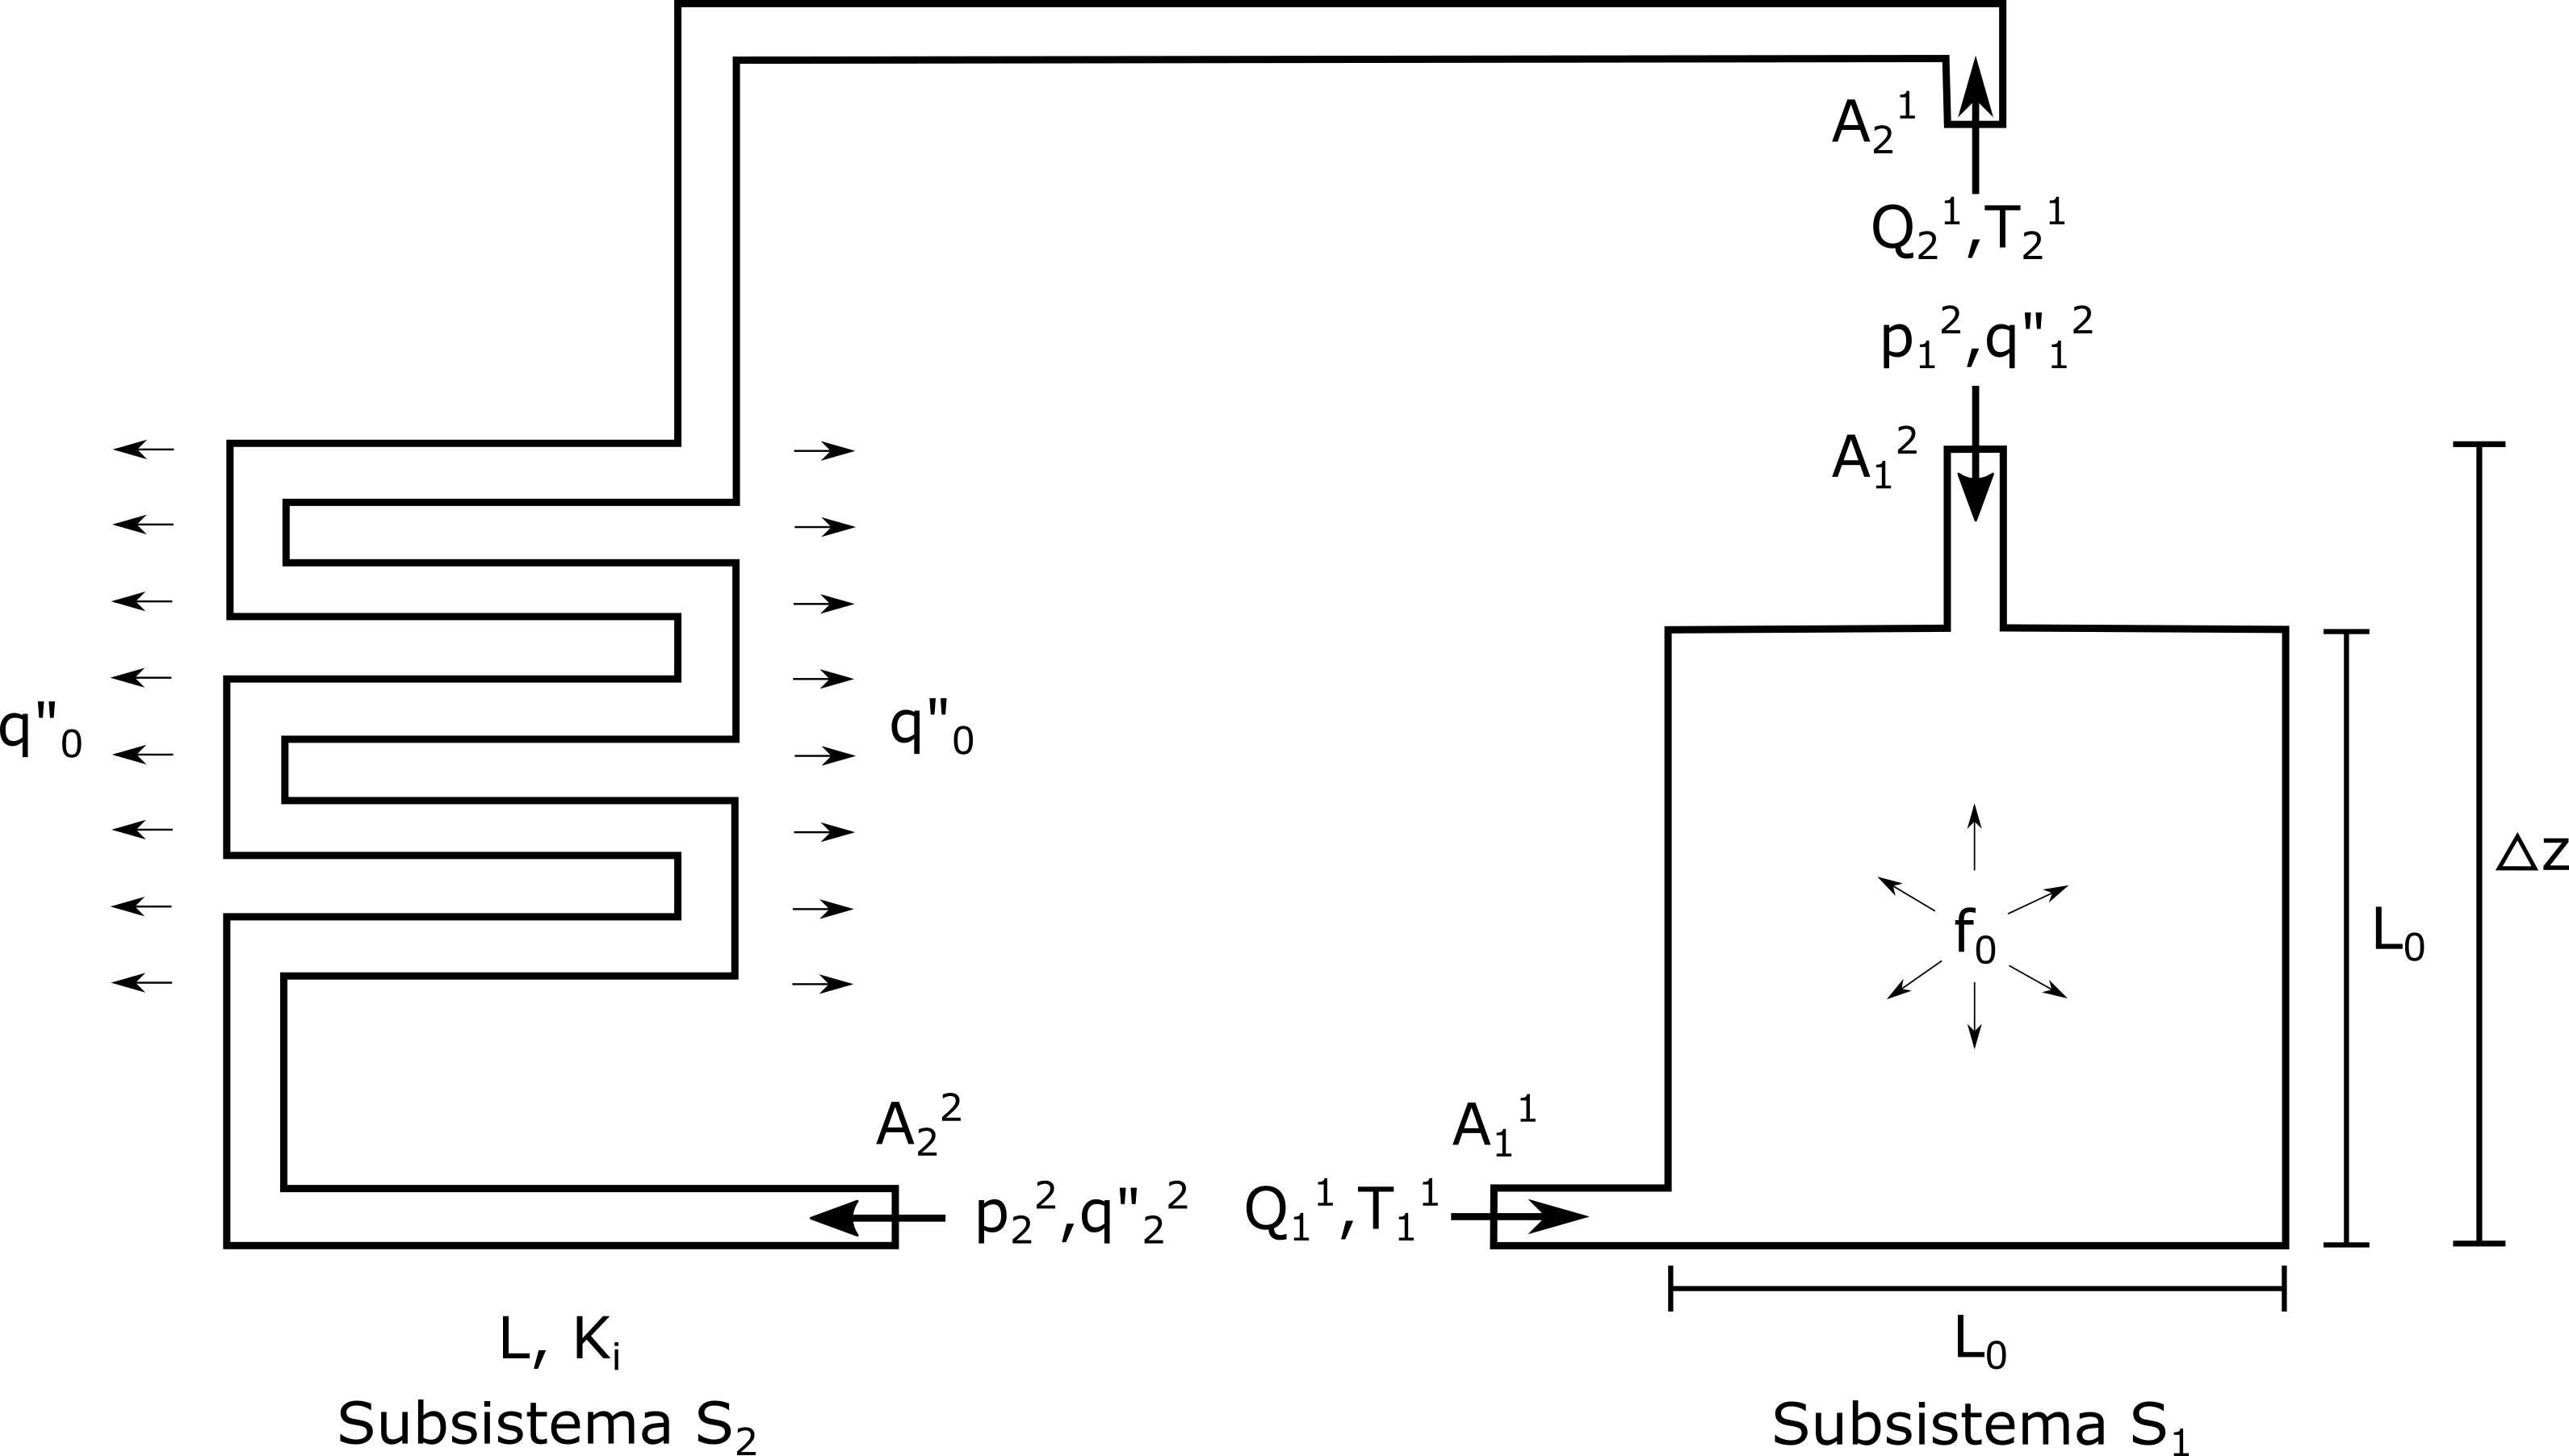
\includegraphics[scale = 0.25]{acople_ri_enief.png}
\caption[Modelo de la fuente fría compuesto por un subsistemas cero-dimensional y otro subsistema bi-dimensional.]
{Modelo de la funete fría analizada. 
El subsistema de la izquierda es un intercambiador de calor y se estudia con un código cero-dimensional.
El modelo de la derecha es una cavidad con una fuente de energía interna y se estudia con un código bi-dimensional.
El sistema completo es abordado con una estrategia de acoplamiento mediante condiciones de borde dinámicas.
En el esquema se ejemplifica una de las elecciones posibles para las variables que son datos en cada subsistema.}
\label{esquemaFuenteFria}
\end{figure}


\subsection*{Subsistemas de estudio}
Los parámetros del modelo del intercambiador de calor son los siguientes:
flujo de calor por unidad de superficie $q_0"=-2\cdot 10^5 W/m^2$, 
longitud de cañerías $L=30$ $m$, 
sumatoria de coeficientes de pérdida de carga concentrada $\sum K_i=1.72$, 
rugosidad de cañerías $\epsilon=0.5\cdot 10^{-3}$ $m$.
Las áreas de las interfaces de acople son $A_2^1=A_2^2=0.03$ $m^2$.
La altura total $\Delta z$ de este subsistema es equivalente a la de la cavidad bidimensional.
El fluido de trabajo es agua ($\rho=10^3$, $c_p=4184$ $J/KgK$).
La evolución de las variables de presión $p$, caudal $Q$ y temperatura $T$ en el subsistema se calcula mediante un código cero-dimensional escrito para este propósito,
que resuelve ecuaciones de pérdida de carga en una red hidráulica con flujo turbulento 
y de transferencia de energía en un intercambiador de calor con flujo constante 
Las ecuaciones del modelo son las siguientes \cite{iedelchik} \cite{kays}:

\begin{equation}
\left\{ \begin{array}{rcl}
p_2^1 + \rho g \Delta z &=& p_2^2 + \rho \frac{1}{2} \left( \frac{Q_1^1}{A_2^1} \right)^2  \left( \frac {f_D L} {D} + \sum_i K_i \right) \\ [0.2cm]
\displaystyle T_2^2 &=& \displaystyle T_2^1 + 2 \frac {q_0" L}{\frac{D}{2} \frac{Q_1^1}{A_2^1}\rho c_p}
\label{eq-intercambiador}
\end{array}
\right.
\end{equation}
donde $p_2^i$ es la presión del subsistema promediada en la interfaz correspondiente,
$Q_2^i$ es el caudal en esta interfaz,
$T_2^i$ es la temperatura promediada en esta interfaz,
$g$ es la aceleración generada por el campo gravitatorio,
$f_D$ es el factor de Darcy de pérdida de carga distribuida,
y $D$ es el diámetro de la tubería.
Notar que el subíndice en cada variable refiere a la numeración global del subsistema, y el supraíndice indica el número de interfaz local,
como se convino previamente en \ref{1:abordaje}.
En este modelo se supone que el flujo de calor es nulo en la dirección axial en cada interfaz de acople.
Esta aproximación es correcta ya que las interfaces se seleccionaron lejos de fuentes y sumideros, donde los gradientes de temperatura son despreciables.
Con este modelo, ninguna de las dos ecuaciones puede recibir valores de contorno \textit{Dirichlet} en ambas interfaces,
ya que los valores de caudal y temperatura en una interfaz determinan el valor en la otra.
Por lo tanto, en la estrategia de acoplamiento, la primera ecuación debe tener, o bien ambos contornos con condiciones de tipo \textit{Neumann}, 
o bien uno con condición de tipo \textit{Neuman} y otro con condición de tipo \textit{Dirichlet}.
La segunda ecuación debe tener uno de los bordes con condición de tipo \textit{Dirichlet} y otro con condición de tipo \textit{Neumann}.
Esta condición es necesaria a pesar de que el flujo de calor recibido no va a ser utilizado, basado en la hipótesis de que es despreciable.
Si el flujo de calor fuera efectivamente apreciable, debería cambiarse el modelo en la ecuación planteada.

La cavidad bidimensional se modela con $L_0=0.3$ $m$, y $A_1^1=A_1^2=0.03$ $m^2$.
Los parámetros del fluido de trabajo son: $\rho_0=10^3$ $Kg/m^3$ a la temperatura de referencia $T_{ref}$,
$\mu=6\cdot 10^{-4}$ $Kg/ms$, $c_p=4184$ $J/KgK$, 
$k=0.64$ $W/mK$ y $\beta=0.44\cdot10^{-3}K^{-1}$.
Se considera que el fluido tiene una fuente interna que se modela como $f_0=10^6$ $W/m^3$.
La evolución de las variables en este subsistema se calcula resolviendo las ecuaciones de Navier-Stokes 
y de transporte de energía.
Se utiliza la aproximación de \textit{Boussinesq} considerando variaciones de densidad solo en el término de fuerza volumétrica.
Las ecuaciones implementadas del modelo son las siguientes \cite{gunzburger} \cite{kays}:

\begin{equation}
\left\{ \begin{array}{rcl}
\displaystyle \frac {\partial \bar{u}}{\partial t} + ( \bar{u} \cdot \nabla) \bar{u}  + \frac {\nabla p}{\rho_0} - 
\nabla \cdot \left[ \left( \nu + \nu_T \right) \left( \nabla \bar{u} + \nabla \bar{u}^T \right) \right] && \\
- \left( 1- \beta (T-T_{ref}) \right)\bar{g} &=& 0 \\ [0.2cm]
\nabla \cdot \bar{u} &=& 0 \\ [0.2cm]
\displaystyle \frac {\partial T}{\partial t} + ( \bar{u} \cdot \nabla) T =0 - \frac {k}{\rho_0 c_p} \Delta T &=& \displaystyle \frac{f_0}{\rho_0 c_p}
\label{eq-cavidad}
\end{array}
\right.
\end{equation}
donde $\bar{u}$ es el campo de velocidades dentro de la cavidad,
$p$ el campo de presiones y
$T$ el campo de temperaturas.

Las ecuaciones (\ref{eq-cavidad}) se resuelven mediante la formulación \textit{Petrov-Galerkin} \cite{galerkin} de elementos finitos, 
con elementos lineales para aproximar los campos de presiones, velocidades y temperaturas, 
estabilizando con los métodos \textit{SUPG} \cite{supg} y \textit{PSPG} \cite{pspg}.
El método \textit{SUPG} (\textit{Streamline Upwind Petrov-Galerkin}) se utiliza para estabilizar problemas de transporte con alto número de \textit{Peclet} (\textit{Pe}).
El \textit{Pe} es un número adimensional que relaciona la velocidad de advección de un flujo y la velocidad de difusión, y está relacionado con el número de \textit{Reynolds} (\textit{Re}).
En las ecuaciones de \textit{Navier-Stokes}, el método estabiliza las evoluciones con alto \textit{Re},
y consiste en la adición de una difusividad extra en la dirección de las líneas de corriente.
El método \textit{PSPG} (Pressure Stabilizing Petrov-Galerkin) se utiliza para evadir la condición \textit{LBB}\footnote{
La condición \textit{Ladyzhenskaya-Babuska-Breezi (LBB)} o \textit{inf-sup}
es una condición necesaria y suficiente para que el problema de \textit{Stokes}
discretizado mediante algún método \textit{Galerkin}
quede bien planteado.
},
que básicamente impone restricciones sobre los espacios de elementos utilizados.

En las paredes se imponen condiciones de no deslizamiento para las ecuaciones de \textit{Navier-Stokes} y de flujo de energía nulo para la ecuación de energía.
En las interfaces de acople, deben definirse una serie de condiciones de borde.
En las ecuaciones de \textit{Navier-Stokes}, en cada interfaz pueden setearse valores de velocidades normales, suponiendo velocidades tangenciales nulas (bajo la hipótesis de flujo paralelo),
o valores de fuerzas normales (presión), suponiendo que las fuerzas tangenciales son nulas.
En la ecuación de energía, cada borde necesita o bien un perfil de temperaturas o bien un perfil de flujo de calor.
Los cálculos se realizaron implementando diferentes estrategias y verificando que los mismos convergieran.

La malla de cálculo se genera con \textbf{Gmsh} \cite{gmsh} y se discretiza el dominio en $43874$ elementos triangulares
con un tamaño medio de arista de $\Delta x \approx 0.005m$.
El cálculo se realiza con \textbf{Par-GPFEP} \cite{gpfep} \cite{pargpfep}.
Las modificaciones de \textbf{Par-GPFEP} que fueron necesarias para implementar el acoplamiento son comentadas en el Apéndice \ref{C:pargpfep}.


\subsection*{Estrategia de resolución}

En cada interfaz de acople existen incógnitas de velocidades, fuerzas, temperatura y flujo de calor.
En el caso de las velocidades la estrategia implementada es definir una variable integral, 
el caudal volumétrico $Q$, que servirá como una de las variables de acoplamiento\footnote{
Cuando se utilizan variables integrales o promediadas para el acoplamiento, es necesario definir una estrategia extra en el subdominio que la recibe.
Como cada subproblema solo queda bien definido si la condición de borde está dada sobre todos los puntos del borde, estos valores deben distribuirse considerando algún perfil.
Por ejemplo, para el caso del subdominio que recibe un valor de caudal, y está modelado con ecuaciones bi-dimensionales, necesita definir un perfil de velocidades a lo largo de toda la sección de acople.
La definición del perfil se basa en alguna hipótesis que el modelador considera adecuada conforme a la física del problema.
Este paso debe analizarse con cuidado ya que los resultados del acoplamiento dependen de ello.
}.
En el caso de las fuerzas se utilizan valores promediados para la fuerza normal (presión $p$).
Las fuerzas tangenciales se consideran nulas bajo la hipótesis de que son despreciables en las interfaces de acople.
Esta hipótesis es correcta cuando el flujo es paralelo, 
y por ello se selecciona como interfaz de acople aquella que se corresponda con el perfil de velocidades lo más plano posible, lejos de las curvas.
Los valores de temperatura de acople también corresponden a valores $T$ promediados en la interfaz,
y el flujo de calor $q''$ de acople corresponde al flujo integral a través de ella.
En los subsistemas bi-dimensionales, los perfiles de velocidadades y temperaturas construidos a partir de las variables recibidas se consideran planos,
bajo la hipótesis de flujo paralelo.
Con esta estrategia, existen cuatro incógnitas en cada interfaz de cada subsistema. 
Considerando los dos subsistemas, existen en total dieciseis incógnitas.

El sistema de ecuaciones de incógnitas queda definido por ocho ecuaciones de continuidad de variables \ref{continuidad}
y otras ocho ecuaciones modelos \ref{ecuaciones-modelos} que todavía deben ser seleccionadas.
Las ecuaciones de continuidad en las interfaces implican que:

\begin{equation}
\left\{ \begin{array}{rcl}
Q_1^1&=& Q_2^2 \\
Q_1^2&=& Q_2^1 \\
p_1^1&=& p_2^2 \\
p_1^2&=& p_2^1 \\
T_2^1&=& T_2^2 \\
T_2^2&=& T_2^1 \\
q"_2^1&=& - q"_2^2 \\
q"_2^2&=& - q"_2^1
\end{array}
\right.
\end{equation}

Las ecuaciones modelos deben ser seleccionadas en base a la combinación de condiciones de borde propuesta para resolver el acoplamiento.
Independientemente de cuál fuera ésta,
para que el problema quede bien planteado debe serleccionarse solo una de las relaciones para el par \textit{presión-caudal}
y solo una para el par ºtextit{temperatura-flujo de calor} en cada interfaz.
Así entonces, considerando las dos interfaces del subsistema 1 se generan cuatro ecuaciones de residuos:

\begin{equation}
\left\{ \begin{array}{rcl}
(R_{p,Q})_{1}^{1}  \;(Q_1^1, p_1^1, T_1^1, Q_1^2, p_1^2, T_1^2) &=& 0 \\
(R_{T,q"})_{1}^{1} \;(Q_1^1, T_1^1, q"_1^1, Q_1^2, T_1^2, q"_1^2) &=& 0 \\
(R_{p,Q})_{1}^{2}  \;(Q_1^1, p_1^1, T_1^1, Q_1^2, p_1^2, T_1^2) &=& 0 \\
(R_{T,q"})_{1}^{2} \;(Q_1^1, T_1^1, q"_1^1, Q_1^2, T_1^2, q"_1^2) &=& 0 
\end{array}
\right.
\label{residuos-1}
\end{equation}
donde $(R_{p,Q})_1^i$ es el residuo del par \textit{presión-caudal} en la interfaz $i$ y
$(R_{T,q''})_1^i$ es el residuo del par \textit{temperatura-flujo de calor} en la interfaz $i$.
Entre las dos interfaces del subsistema 2 se generan otras cuatro ecuaciones de residuos:

\begin{equation}
\left\{ \begin{array}{rcl}
(R_{p,Q})_{2}^{1}  \;(Q_2^1, p_2^1, T_2^1, Q_2^2, p_2^2, T_2^2) &=& 0 \\
(R_{T,q"})_{2}^{1} \;(Q_2^1, T_2^1, q"_2^1, Q_2^2, T_2^2, q"_2^2) &=& 0 \\
(R_{p,Q})_{2}^{2}  \;(Q_2^1, p_2^1, T_2^1, Q_2^2, p_2^2, T_2^2) &=& 0 \\
(R_{T,q"})_{2}^{2} \;(Q_2^1, T_2^1, q"_2^1, Q_2^2, T_2^2, q"_2^2) &=& 0
\end{array}
\right.
\label{residuos-2}
\end{equation}
Notar que según la estrategia de acoplamiento seleccionada, algunas de las dependencias pueden anularse.
En la Figura \ref{esquemaFuenteFria} se presenta una estrategia en la que las condiciones de borde dinámicas son 
de tipo de tipo Dirichlet para la interfaz inferior de la cavidad y la interfaz superior del intercambiador de calor, 
y de tipo de tipo Neumann para las restantes.

Como el circuito es cerrado es necesario proveer un valor de referencia para la presión.
En la formulación desarrollada se fija un valor de presión aritrario en la interfaz superior del intercambiador de calor,
por lo que la ecuación $(R_{p,Q})_{2}^{1}=0$ queda descartada, y es sustituida por la siguiente:

\begin{equation*}
p_2^1 = 0.
\end{equation*}

El programa \textit{maestro} utilizado es \textbf{Coupling}.
La comunicación entre códigos se da por MPI en modo SISD.
Como se mencionó en \ref{1:evolucion}, no existe necesidad de que ambos códigos utilicen el mismo paso temporal de cálculo.
Sin embargo en ambos modelos se utiliza $\Delta t=0.01s$, debido a que ninguno requiere una mayor discretización temporal.

\subsection*{Resultados del cálculo}

\begin{figure}[ht]
	\begin{minipage}{0.5\linewidth}
		\centering
		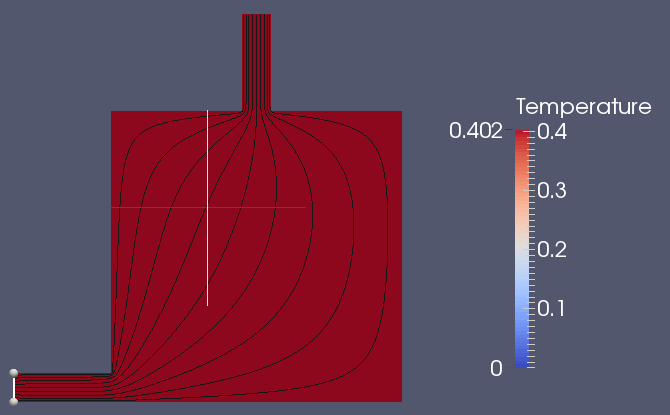
\includegraphics[scale=0.32]{acople_ri28_t0.png}
		\caption[]{t=0 s}
		\label{asd}	
	\end{minipage}
	\begin{minipage}{0.5\linewidth}
		\centering
		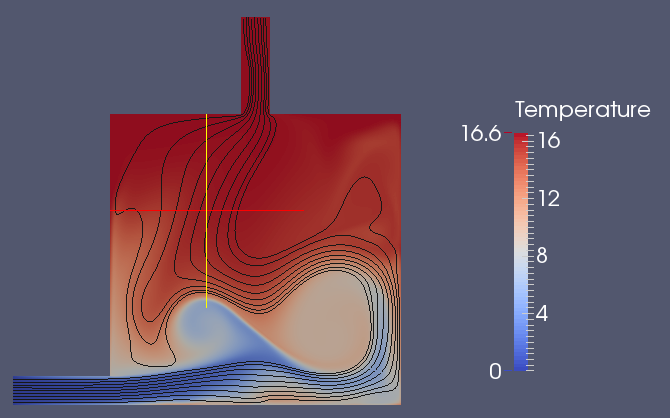
\includegraphics[scale=0.315]{acople_ri28_t40.png}
		\caption[]{t=40 s}
		\label{asd}	
	\end{minipage}
	\caption[Evolución en el transitorio inicial del fluido dentro de la cavidad bidimensional con fuente interna]
  {Evolución del fluido dentro de la cavidad bidimensional con fuente interna.
	El número de Richardson del fluido $Ri=28.34$.
	Pueden apreciarse las líneas de corriente que se establecen al comienzo de la simulación.} 
	\label{acople_ri28_1}
\end{figure}

\begin{figure}[ht]
	\begin{minipage}{0.5\linewidth}
		\centering
		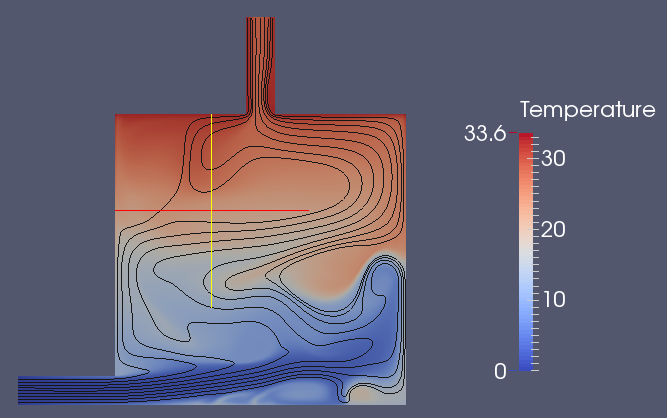
\includegraphics[scale=0.32]{acople_ri28_t80.png}
		\caption[]{t=80 s}
		\label{asd}	
	\end{minipage}
	\begin{minipage}{0.5\linewidth}
		\centering
		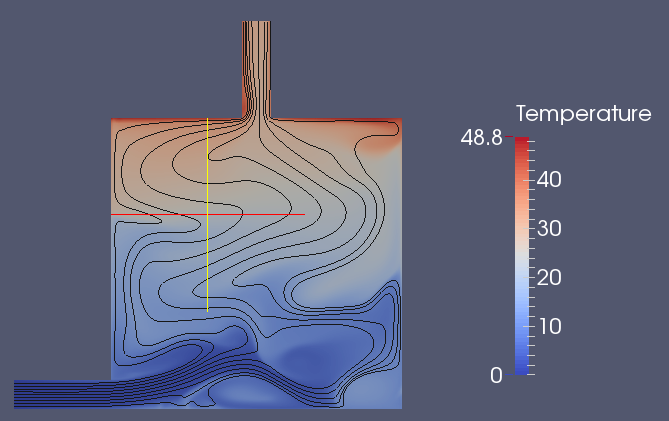
\includegraphics[scale=0.315]{acople_ri28_t250.png}
		\caption[]{t=250 s}
		\label{asd}	
	\end{minipage}
	\caption[Evolución hacia el estado estacionario del fluido dentro de la cavidad bidimensional con fuente interna]
  {Evolución del fluido dentro de la cavidad bidimensional con fuente interna.
	El número de Richardson del fluido $Ri=28.34$.
	Pueden apreciarse las líneas de corriente serpenteantes y la estratificación del fluido alcanzando un estado estacionario.}  
	\label{acople_ri28_2}
\end{figure}

Las condiciones iniciales del sistema son estáticas y sin gradientes de temperatura.
A medida que evoluciona el fluido comienza a incrementar su temperatura en la cavidad y a circular por fuerza boyante.
El régimen del fluido depende del número adimensional de Richardson \textit{Ri}, \cite{richardson},
que representa la relación entre las fuerzas boyantes y las fuerzas inerciales.
Con los parámetros del subsistema bidimensional el \textit{Ri} del fluido queda definido en $Ri=28.34$.
Como este valor es alto, el fluido se estratifica en capas de diferentes temperaturas.
Las líneas de corrientes serpentean entre la entrada y la salida, manteniendo corrientes paralelas horizontales.
En las Figuras \ref{acople_ri28_1} y \ref{acople_ri28_2} puede observarse 
la evolución de las líneas de corriente y del campo de temperatura en la cavidad bidimensional.

\subsection*{Análisis de métodos de resolución del sistema de ecuaciones de residuos}

Se exploran diferentes métodos numéricos para resolver el acoplamiento presentado en las ecuaciones \ref{residuos-1} y \ref{residuos-2}.
El parámetro de interés aquí no es la cantidad de iteraciones de cada método sino la cantidad de evaluaciones de funciones que cada uno requiere,
ya que el tiempo de cálculo está directamente relacionado con ellas.
En la Figura \ref{iteraciones_ri} puede apreciarse la cantidad de evaluaciones requeridas 
por cada método para disminuir los residuos debajo de cierta tolerancia prefijada, para cada paso temporal.
El método de \textit{Newton} calcula la matriz jacobiana en cada iteración.
Este cálculo se realiza con diferencias finitas a primer órden y por lo tanto requiere 1 evaluación de los residuos en el punto inicial, y 8 evaluaciones extras para el cálculo de cada diferencia finita.
En total son 9 evaluaciones extras.
Puede observarse que la cantidad de iteraciones del método para converger es en promedio una sola, ya que en general utiliza 10 evaluaciones en cada paso temporal.

\begin{figure}[ht]
\centering{}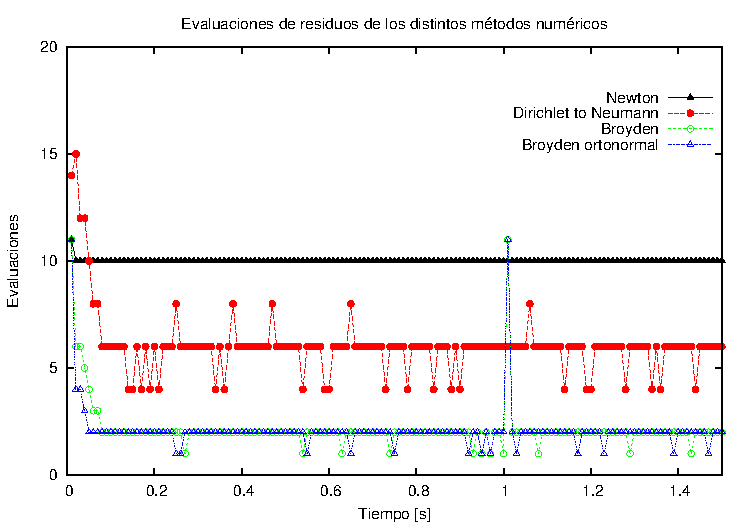
\includegraphics[scale = 1]{evaluaciones-ff.pdf}
\caption
{Evaluaciones de residuos requeridas por diversos métodos numéricos para resolver los sistemas de ecuaciones planteados
 en el problema doblemente acoplado descripto de la fuente fría de neutrones.} \label{iteraciones_ri} 
\end{figure}

Los métodos \textit{quasi-Newton} inicializan la matriz jacobiana sólo en el primer paso temporal,
y luego utilizan aproximacionas económicas de la misma. 
Cada cierta cantidad de pasos temporales pueden reinicializar la matriz también mediante diferencias finitas. 
En los modelos realizados se utiliza reinicialización cada 100 pasos temporales, 
y por lo tanto la primera reinicialización se efectúa en el paso 101.
En promedio estos métodos requieren dos iteraciones por cada paso temporal, 
además de las 9 llamadas extras a códigos en cada paso de reinicialización.
Los métodos \textit{Broyden} y \textit{Broyden ortonormal} tinen comportamiento similar y demuestran ser más eficientes que el método clásico.
El método \textit{Dirichlet-to-Neumann} es el que mayor cantidad de iteraciones necesita por cada paso temporal, 
excediendo el doble de los pasos requeridos por los métodos \textit{quasi-Newton}.

\section{Análisis del segundo sistema de parada de un reactor de investigación}
\label{3:mockup}

\subsection*{Presentación del problema}
El Departamento de Mecánica Computacional de CNEA tuvo a cargo el análisis del segundo sistema de parada (SSP) del reactor RA-10 \cite{ra10}.
El RA-10 es un reactor de investigación multipropósito, destinado principalmente a aumentar la producción de radioisótopos para uso de diagnóstico de enfermedades,
a la investigación científica de haces de neutrones en diferentes rangos de energía,
y al ensayo de materiales.
El RA-10 es un reactor de pileta abierta de flujo ascendente, con combustibles de bajo enriquecimiento tipo placa y agua liviana como refrigerante.
El núcleo del reactor está inmerso en un tanque que contiene agua pesada como material reflector.
El SSP consiste en el accionamiento del vaciado este tanque.
El drenado del agua pesada disminuye drásticamente la reactividad, apagando el reactor.
La tarea de estudio consistió en verificar si el diseño cumple con el criterio de éxito,
a saber, completar el 55\% del vaciado en un tiempo inferior a los 15 segundos,
ante una falla simple del sistema (falla de apertura de cualquiera de las válvulas).
Este requerimiento pudo verificarse tras el análisis \cite{cnea-informe-ra10}.

\begin{figure}[ht]
\centering{}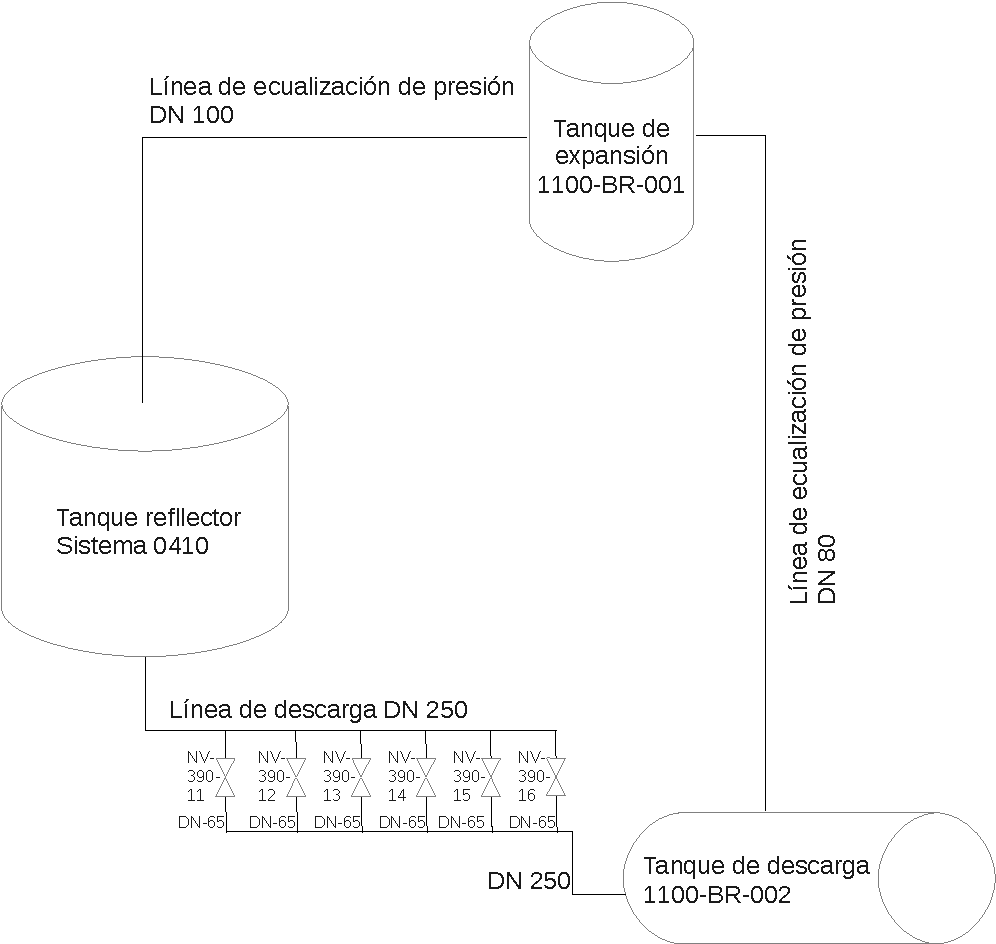
\includegraphics[scale = 0.8]{SSP.pdf}
\caption{Esquema del segundo sistema de parada del reactor RA10.} \label{fig:SSP} 
\end{figure}

La Figura \ref{fig:SSP} esquematiza el SSP. 
En el mismo pueden destacarse tres grandes subsistemas: el tanque del reflector, la red hidráulica de descarga y
la red hidráulica de ecualización de presiones. 
En operación normal del reactor las
válvulas que pueden observarse en la red hidráulica permanecen cerradas, y el agua pesada rellena las cañerías y el tanque de reflector. 
El resto del sistema es rellenado con gas Helio, excepto una porción del tanque de expansión que también permanece rellena con líquido. 
Cuando es accionado el SSP se abren las válvulas y el líquido comienza a drenar hacia el tanque de descarga, acelerado por la fuerza gravitatoria. 
Asimismo, el Helio circula en el mismo sentido en el resto del sistema, rellenando el volumen desplazado de líquido.

El análisis del problema completo hubiera demandado elevados recursos computacionales debido a los requerimientos de malla.
Por ello se propuso desarrollar un modelo multiescala del sistema,
desacoplándolo en subsistemas que pudieron estudiarse por separado con estrategias de acoplamiento mediante condiciones de borde apropiadas.
El SSP del RA10 se dividió en tres subsistemas:

\begin{itemize}
\item Subsistema del tanque del reflector,
\item Subsistema de la red hidráulica de descarga,
\item Subsistema de la red hidráulica de ecualización de presiones.
\end{itemize}

En el trabajo presentado los subsistemas se acoplaron mediante una estrategia de acoplamiento débil \cite{ra10-paper} \cite{ra10-enief}.

Previo a este trabajo, se realizaron tareas de validación de las herramientas de cálculo.
Para ello se estudió un sistema similar para el que se conocían datos experimentales de tiempo de vaciado.
Estos datos sirvieron para contrastar los resultados obtenidos con las herramientas de cálculo.
El sistema analizado fue el \textit{mockup} del SSP del reactor OPAL \cite{invap-mockup},
montado por INVAP en San Carlos de Bariloche.
Debido a que el \textit{mockup} del SSP del OPAL está abierto a la atmósfera,
no cuenta con línea de ecualización de presiones y por lo tanto ésta no se consideró en el modelo.
En un estudio \cite{cnea-informe-mockup} se analizó el detalle fluídico tridimensional en el tanque reflector durante la descarga,
modelando con ecuaciones cero-dimensionales la pérdida de carga en la red hidráulica 
y acoplando los subsistemas de forma débil.
El estudio que a continuación se presenta es otro estudio que analiza con mayor detalle la distribución de caudales a través del arreglo de válvulas,
modelando el comportamiento del resto del sistema con ecuaciones cero-dimensionales,
y acoplando los subsistemas de forma fuerte, con la estrategia descripta en los dos primeros capítulos.
El propósito de este estudio es investigar si existe algún efecto en las cañerías que podría no estar siendo considerado en el otro modelo.

\subsection*{Subsistemas de estudio}

Se proponen dos subsistemas de estudio:
el primero incluye el tanque del reflector acoplado a una porción de la red hidráulica en la descarga,
y el segundo modela el arreglo de válvulas.

El primer subsistema se analiza con ecuaciones cero-dimensionales,
realizando balances de masa y energía.
La evolución de la altura $h$ de la superficie libre en el tanque del reflector
queda modelada a través de la siguiente ecuación \cite{bird}:

\begin{equation}
\ddot{h} h + \frac{\dot{h}^2}{2}\left( 1- \left(\frac{A_T}{A_D} \right)^2 \right) + g \Delta h_{red} + \ddot{h}  l_D = 
\frac{p_{atm}-p_1^1}{\rho} + \Delta \hat{u}
\label{eq-tanque}
\end{equation}
donde $p_1^1$ es la presión en la interfaz de acople,
$A_T$ es la área transversal del tanque del reflector, 
$A_D$ es la sección transversal de la línea de descarga,
$\Delta h_{red}$ es la altura total de la columna de líquido en el subsistema,
$l_D$ es la longitud total de cañerías en el subsistema,
$p_{atm}$ es la presión sobre la superficie libre,
y $\rho$ es la densidad del agua.
$\Delta u$ representa la pérdida de carga por unidad de masa y puede modelarse como:

\begin{equation}
\Delta u = \frac {1} {2} {v_D}^2 \left( \frac {f_D l_D}{D} + \sum_i K_i \right)
\end{equation}
donde $v_D$ es la velocidad del fluido en la línea de descarga,
(que puede escribirse en términos de $\dot{h}$),
$\frac {f_D*l_D}{D}$ es el factor de pérdida de carga distribuida en las tuberías,
(en función del factor de Darcy $f_D$, la longitud de tuberías $l_D$ y el diámetro de las mismas $D$)
y $\sum_i K_i$ es la sumatoria de factores de pérdida de carga concetrada.

La Tabla \ref{tabla-tanque} reúne los parámetros del subsistema.
Los datos geométricos pueden consultarse en las referencias \cite{invap-mockup}.
El factor de pérdida de carga concentrada fue calculado en función de estos datos geométricos \cite{iedelchik},
e incluye la contracción abrupta en la unión entre el tanque y la red hidráulica,
y tres codos de 90º presentes en ella, previos al arreglo de válvulas.

\begin{table}[]
\centering
\begin{tabular}{|l|l|}
\hline
Parámetro        & Valor          \\ \hline
$A_T$            & 5.30 $m^2$     \\ \hline
$A_D$            & 0.05 $m^2$     \\ \hline
$\Delta h_{red}$ & $h$ + 4.98 $m$ \\ \hline
$l_D$            & 11.98 $m$      \\ \hline
$p_{atm}$        & 92000 $Pa$     \\ \hline
$\rho$           & 998 $Kg/m^3$   \\ \hline
$D$              & 0.254 $m$      \\ \hline
$\sum_i K_i$     & 1.13           \\ \hline
\end{tabular}
\caption{Parámetros del subsistema del tanque del reflector con acople de sección de red hidráulica}
\label{tabla-tanque}
\end{table}

Una vez resuelta la ecuación (\ref{eq-tanque}) para un dado valor de tiempo,
el caudal de descarga $Q_1^1$ puede calcularse simplemente como:

\begin{equation}
Q_1^1 = -\dot{h} A_D
\label{eq-qd}
\end{equation}
Todos estos cálculos se realizan con un programa escrito para este propósito.

El subsistema arreglo de válvulas es modelado con una malla tridimensional de elementos tetraédricos realizada en \textbf{Salomé} \cite{salome}.
El caudal ingresa a través del extremo superior y se reparte entre los múltiples caños que comunican los colectores.
En operación normal del reactor cada uno de ellos está bloqueado mediante una válvula esférica,
y del otro lado las cañerías están rellenas de gas,
pero durante el accionamiento del sistema de parada las mismas se abren dejando pasar libremente al fluido.
Las válvulas esféricas instaladas no presentan pérdidas de carga concentrada y por lo tanto no son modeladas.
Como es de interés el análisis ante falla simple del sistema,
se supone que una de las válvulas no abre y por ello ese caño tampoco se modela.
En los primeros cálculos se supone que la válvula en falla es la ubicada en la última rama del arreglo.
Como otra simplificación del problema se supone que inicialmente el agua rellena todas las cañerías en forma estática.
Más adelante se estudia la validez de éstas aproximaciones.
Los datos dimensionales de las cañerías pueden consultarse en las referencias \cite{invap-mockup}.

Debido a que el régimen del fluido es turbulento durante la mayor parte de la descarga,
y una simulación DNS (Simulación Numérica Directa, por sus siglas en inglés \textit{Direct Numerical Simulation} demandaría elevados recursos computacionales,
se utiliza un modelo de turbulencia de tipo RANS (Promedio de Reynolds de Navier-Stokes, por sus siglas en inglés \textit{Reynolds-Averaged Navier–Stokes})
para modelar la fricción interna del fluido.
El modelo utilizado es el modelo $\kappa-\epsilon$ \textit{realizable} \cite{k-e-realizable},
en el que las ecuaciones se estabilizan mediante un método de control de coeficiente.
El sistema de ecuaciones resultantes en el segundo subsistema es:

\begin{equation}
\left\{ \begin{array}{rcl}
\displaystyle \frac{\partial \bar{U} }{\partial t} + ( \bar{U} \cdot \nabla) \bar{U} + \frac {\nabla P^*}{\rho} - 
\nabla \cdot \left[ \left( \nu + \nu_T \right) \left( \nabla \bar{U} + \nabla U^T \right) \right] -\bar{f} &=& 0 \\
\nabla \cdot \bar{U} &=& 0 \\
\displaystyle \nu_T -c_\mu \frac{\kappa^2}{\epsilon} &=& 0\\
\displaystyle \frac{\partial \kappa}{\partial t} + ( \bar{U} \cdot \nabla) \kappa - \frac{c_\mu} {2}{\kappa^2}{\epsilon} \left | \nabla \bar{U} + \nabla\bar{U}^T \right | ^2  
- \nabla \cdot \left( c_\mu \frac{\kappa^2}{\epsilon} \nabla \kappa \right) + \epsilon &=& 0 \\
\displaystyle \frac{\partial {\epsilon}}{\partial t} + ( \bar{U} \cdot \nabla) \epsilon - \frac{c_1} {2} \kappa \left | \nabla \bar{U} + \nabla \bar{U}^T \right | ^2
- \nabla \cdot \left( c_{\epsilon} \frac{\kappa^2}{\epsilon} \nabla \epsilon \right) + c_2 \frac{\epsilon}{\kappa} &=& 0
\label{eq-mani}
\end{array} \right.
\end{equation}
donde $\bar{f}$ es una fuerza volumétrica, 
$\kappa$ es la energía cinética turbulenta, $\epsilon$ es la disipación viscosa de energía turbulenta,
$\nu_T$ es la viscosidad turbulenta y $P^*$ es la presión efectiva del sistema, que se calcula como
$\displaystyle P^* = P + \frac {2}{3}\kappa$.
Las variables mayúsculas refieren a valores medios estadísticos.
Los parámetros de las ecuaciones de transporte de $\kappa$ y $\epsilon$ toman los siguientes valores:
$c_\mu=0.09$, $c_1=0.126$, $c_2=1.92$ y $c_\epsilon=0.07$ \cite{durbin}.

En las ecuaciones de \textit{Navier-Stokes}, cada borde necesita un perfil de velocidades normales o de fuerzas normales,
y otro de velocidades tangenciales o de fuerzas tangenciales \cite{gunzburger}.
Si la condición de borde de ingreso de la cañería es el valor del caudal $Q_2^1$,
a partir de éste puede definirse un perfil de velocidades del fluido.
El regímen de flujo es turbulento durante la mayor parte de la descarga y por tanto este perfil puede suponerse plano.
En base a estas velocidades puede calcularse un valor para la intensidad turbulenta $I_T$,
y con ella aproximarse los valores de $\kappa$ y $\epsilon$ en la interfaz.
Si la condición de borde de ingreso a la cañería es el valor de presión media,
la intensidad turbulenta $I_T$ en cada paso de evolución temporal puede calcularse de forma aproximada a partir de la solución para el caudal en el paso previo.
En la descarga de la cañería se impone una fuerza normal que depende de la presión atmosférica,
despreciando las fuerzas tangenciales.
Las ecuaciones de $\kappa$ y $\epsilon$ no requieren condiciones de contorno en esta interfaz.
Para evitar la resolución de la capa límite en las paredes de las tuberías se implementa un modelo de pared,
en el que se reemplaza la misma por una tracción tangencial equivalente a la que realizaría la misma sobre la corriente externa
\cite{k-e}.
Este modelo impone condiciones de tipo \textit{Dirichlet} para $\kappa$ y $\epsilon$ en la frontera en que se impone la ley de pared.

El sistema de ecuaciones (\ref{eq-mani}) es resuelto en pasos fraccionados \cite{lew} mediante la formulación \textit{Petrov-Galerkin} \cite{galerkin} de elementos finitos con elementos lineales, 
estabilizada mediante \textit{SUPG} \cite{supg} y \textit{PSPG} \cite{pspg}.
En el primer paso fraccionado se resuelve el transporte de $\kappa$,
en el segundo paso se resuelve el transporte de $\epsilon$,
y en el último paso se resuelven en forma monolítica las ecuaciones de \textit{Navier-Stokes}.

Una vez resueltas las ecuaciones,
si la condición de borde en la interfaz de acople $I_{2_1}$ había sido el caudal $Q_2^1$,
es posible calcular el valor de la presión promedio $<p_2^1>$ en esta interfaz
a partir de los valores $<P^*_{I_2^1}>$ y $<\kappa_{I_2^1}>$ promediados en ella:

\begin{equation}
<p_2^1> = <P^*_{I_2^1}> - \frac {2}{3} <\kappa_{I_2^1}>
\end{equation}

Si la condición de borde en la interfaz de acople hubiera sido la presión promedio $<p_2^1>$,
el caudal $Q_2^1$ se calcula simplemente mediante integración numérica del campo de velocidades en los nodos de la interfaz.

Todos estos cálculos se realizan con \textbf{Par-GPFEP}.

\subsection{Estrategia de resolución}

Los dos subsistemas están conectados a través de una sección de la tubería,
en la cual quedan acoplados los valores de velocidades y fuerzas.
La estretegia implementada es similar a la utilizada en \ref{3:ff} y consiste en utilizar como variables de acoplamiento el caudal volumétrico $Q$ y la presión promedio $p$.
Las fuerzas tagenciales se consideran nulas.
A fines de cumplir con esta hipóteisis, la interfaz de acople se selecciona lejos de los codos.
El subsistema tanque del reflector tiene como incógnitas la presión $p_1^1$ y el caudal $Q_1^1$ en la interfaz de acople $I_1^1$.
Asimismo, el subsistema arreglo de válvulas tiene como incógnitas $p_2^1$ y $Q_2^1$ en $I_{2_1}$.
Las ecuaciones de continuidad implican que:

\begin{equation}
\left\{ \begin{array}{rcl}
p_1^1 &=& p_2^1 \\
Q_1^1 &=& Q_2^1
\end{array}
\right.
\end{equation}

Se utiliza la siguiente estrategia:
condiciones de borde de tipo \textit{Neumann} en la interfaz de acople para el subsistema tanque del reflector,
y condiciones de borde de tipo \textit{Dirichlet} para el subsistema arreglo de válvulas\footnote{
Se podrían haber definido otras estrategias.
La estrategia implementada permite resolver las ecuaciones en ambos subdominios de una forma cómoda.
En el modelo tri-dimensional, por ejemplo, el valor de caudal recibido es útil para construir valores para las condiciones de borde del modelo turbulento utilizado.
}.
En base al caudal recibido en este subsistema se calcula un perfil de velocidades.
Las ecuaciones de residuos quedan entonces:

\begin{equation}
\left\{ \begin{array}{rcl}
(R_{p,Q})_{1}^{1}  \;(p_1^1) &=& 0 \\
(R_{p,Q})_{2}^{1}  \;(Q_2^1) &=& 0
\end{array}
\right.
\end{equation}

El programa \textit{maestro} utilizado es \textbf{Coupling}.
La comunicación entre códigos se da por MPI en modo SIMD.

\subsection*{Evolución de la descarga del SSP}

Se realizan cálculos utilizando mallas del modelo tri-dimensional con diferente refinamiento para estudiar la convergencia de los resultados.
La primera es una malla con $\Delta x=0.01m$ y 1145659 de elementos. 
La segunda es malla tiene $\Delta x=0.008m$ y 1806202 elementos.
La tercera es la malla más fina y tiene $\Delta x=0.005m$ y 2951259 elementos.
Se utiliza $\Delta t=0.01s$ en los cálculos con las dos primeras mallas y $\Delta t=0.005s$ en los cálculos con la última malla.
Las ecuaciones de residuos se resuelven
mediante el método de \textit{Broyden ortonormal},
con reinicialización de la matriz jacobiana cada 100 pasos temporales.
En la Figura \ref{qpvst} se reportan los resultados obtenidos para la evolución de los caudales y de las presiones en la interfaz de acople.

\begin{figure}[ht]
	\begin{minipage}{0.5\linewidth}
		\centering
		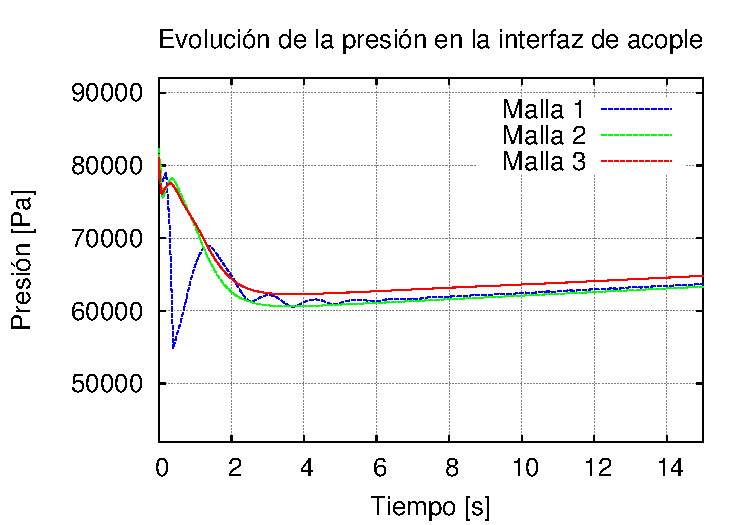
\includegraphics[scale=0.55]{p_vs_t.pdf}
		%\caption{t=80 s}
		\label{asd}	
	\end{minipage}
	\begin{minipage}{0.5\linewidth}
		\centering
		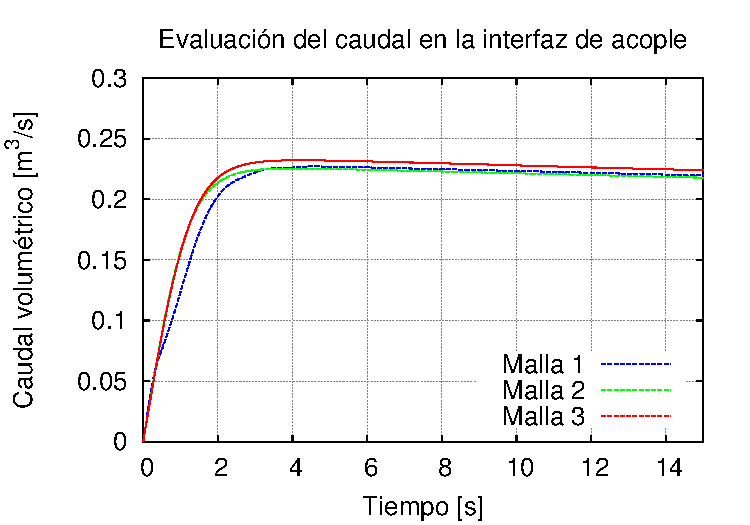
\includegraphics[scale=0.55]{q_vs_t.pdf}
		%\caption{t=250 s}
		\label{asd}	
	\end{minipage}
	\caption[Evolución de la presión y del caudal volumétrico en la interfaz de acople]
  {Evolución de la presión y del caudal volumétrico en la interfaz de acople entre los dos subsistemas.
  La presión atmosférica es de 92000 Pa.}  
	\label{qpvst}
\end{figure}

%~ \begin{figure}[ht]
%~ \centering{}\includegraphics[scale = 1]{qpvst.pdf}
%~ \caption{Evolución de la presión y del caudal volumétrico en la interfaz de acople entre los dos subsistemas.}
%~ \label{qpvst}
%~ \end{figure}

En la Figura \ref{hvst} se observa la evolución de la altura de la superficie libre del líquido en el tanque durante los primeros quince segundos obtenida en diferentes cálculos.
La curva azul reporta los resultados obtenidos con la malla más gruesa, la curva roja los resultados obtenidos con la malla intermedia y la curva violeta los resultados obtenidos con la malla más fina.
La curva verde muestra resultados de análisis estudiando la condición inicial de gas de relleno en las cañerías, que será descripta en la sección \ref{3:level-set}.
Las curvas cyan y gris muestran resultados del cálculo del modelo tri-dimensional del tanque con acoplamiento débil al modelo cero dimensional de la red hidráulica \cite{ra10-paper}.
La primera curva fue obtenida sin utilizar modelo de turbulencia, y la segunda utilizando el modelo RANS previamente comentado.
Comparativamente se muestran también los valores experimentales reportados en la referencia \cite{invap-mockup}.

\begin{figure}[ht]
\centering
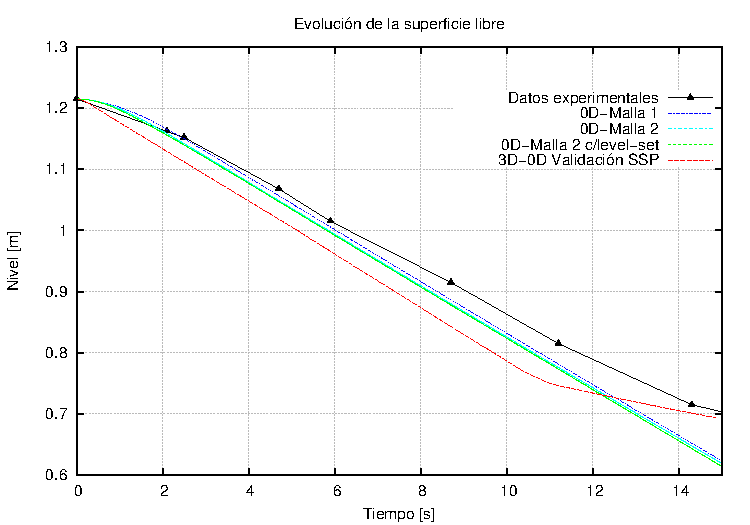
\includegraphics[scale = 1]{hvst.pdf}
\caption[Evolución del nivel de líquido en el \textit{mockup} del tanque del reflector del reactor OPAL ante accionamiento del SSP]
{Evolución del nivel de líquido en el \textit{mockup} del tanque del reflector del reactor OPAL ante accionamiento del SSP.
La curva negra está construida con datos experimentales proporcionados por INVAP S.E.
Las curvas azul, roja, verde y violeta reportan datos calculados mediante diferentes mallas para el modelo tri-dimensional del arreglo de válvulas, 
con acoplamiento fuerte al modelo cero-dimensional del resto del sistema.
Las curvas cyan y gris muestran resultados del cálculo del modelo tri-dimensional del tanque con acoplamiento débil al modelo cero dimensional de la red hidráulica.}
\label{hvst} 
\end{figure}

Los modelos computacionales predicen un comportamiento dinámico similar al reportado experimentalmente.
Durante los primeros segundos de evolución existe una cierta inercia en la descarga que solo es captada por los modelos que describen el detalle en el arreglo de válvulas.
Tras este transitorio inicial, todos los modelos predicen una pendiente de vaciado similar.
Esta pendiente se corresponde con similares caudales de descarga entre los diferentes modelos, 
con lo que se verifica que la pérdida de carga total considerada en dos modelos independientes (modelo tri-dimensional del tanque acoplado, y modelo cero-dimensional del tanque acoplado) es similar.
La curva experimental presenta ciertas ondulaciones que se deben al efecto que el oleaje en la superficie del líquido genera sobre el punto de medición.
Estas variaciones son filtradas en los modelos utilizados, 
ya que las curvas calculadas reportan alturas efectivas, computadas a partir del volumen restante de líquido en el tanque.
Transcurridos diez segundos de evolución, existe un quiebre en las curvas del modelo tri-dimensional del tanque.
Este quiebre se corresponde al momento en el que las cañerías succionan tanto gas que es posible desacoplar el modelo cero-dimensional de pérdida de carga,
basándose en la hipótesis de que se establece una vena gaseosa entre el punto de succión y el orificio de descarga.
Esta hipótesis es conservativa para el objetivo de estudio previsto,
ya que si el acoplamiento de la red no fuera realmente despreciable, el tanque se vaciaría a mayor velocidad que la modelada.
En el tanque existe un cajón que envuelve la entrada a la red hidráulica y no permite el vaciado más allá de los 60 cm,
por lo que el nivel de líquido, que es medido fuera de este cajón, tiende asintóticamente a este valor.
Esta dinámica no es considerada en el modelo cero-dimensional del tanque, lo que explica las diferencias entre las curvas en los últimos segundos.

\subsection*{Análisis de sensibilidad de resultados ante válvula en falla}

Los cálculos previos se realizaron suponiendo que falla la válvula de la última conexión entre los colectores.
Es de interés conocer si existe variación en los tiempos de descarga si la válvula que falla es alguna otra.
En la Figura \ref{hvstv} se compara la evolución de la superficie libre ante fallas en la primera, la tercera y la sexta válvula.

\begin{figure}[ht]
\centering
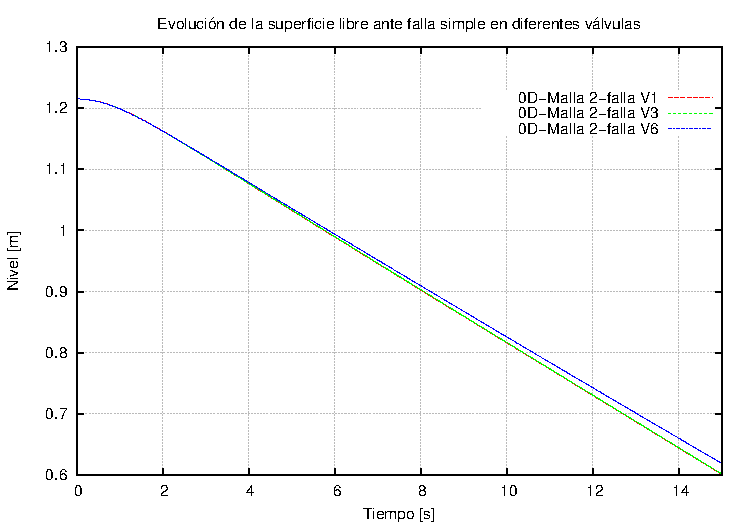
\includegraphics[scale = 1]{hvstv.pdf}
\caption[Evolución del nivel de líquido en el \textit{mockup} del tanque del reflector del OPAL ante accionamiento del SSP considerando falla simple en diferentes válvulas]
{Evolución del nivel de líquido en el \textit{mockup} del tanque del reflector del OPAL ante accionamiento del SSP considerando falla simple en diferentes válvulas.}
\label{hvstv} 
\end{figure}

Como puede observarse no es posible notar diferencias considerables en la evolución.
La pérdida de carga total del arreglo de válvulas es levemente sensible a la válvula que falla.

\subsection*{Transporte de superficie libre en las tuberías}
\label{3:level-set}

Como se comentó, en los cálculos realizados previamente no se consideró el gas de relleno en las tuberías durante los primeros instantes del drenado.
Es de interés estudiar su influencia.
Se utiliza la técnica de level-set para transportar la superficie libre \cite{level-set}.
Para ello se añade un paso fraccionado extra al sistema de ecuaciones (\ref{eq-mani}):

\begin{equation}
\left\{ \begin{array}{rcl}
\displaystyle \frac{\partial\phi}{\partial t}+ (\bar{u} \cdot \nabla) \phi &=& 0
\label{eq-ls}
\end{array} \right.
\end{equation}
donde $\phi$ es el campo que representa la distancia con signo de cada punto a la superficie libre.
Las porciones del sistema con líquido tienen $\phi$ positivo y las porciones con gas tienen $\phi$ negativo.
$\phi$ tiene valor nulo en la superficie libre.
La ecuación (\ref{eq-ls}) requiere un valor de contorno allí donde $\bar{u} \cdot \bar{n} < 0$,
y por lo tanto debe proveerse el valor del campo a la entrada de la tubería.
Esta ecuación también es resuelta mediante una formulación de elementos finitos con elementos lineales y estabilización \textit{SUPG}.
Se utiliza, además, un enriquecimiento del espacio de presiones en los elementos de la interfaz \cite{enriq}.
El campo del level set es reinicializado mediante cálculos geométricos cada 10 pasos temporales.

\begin{figure}[ht]
\centering
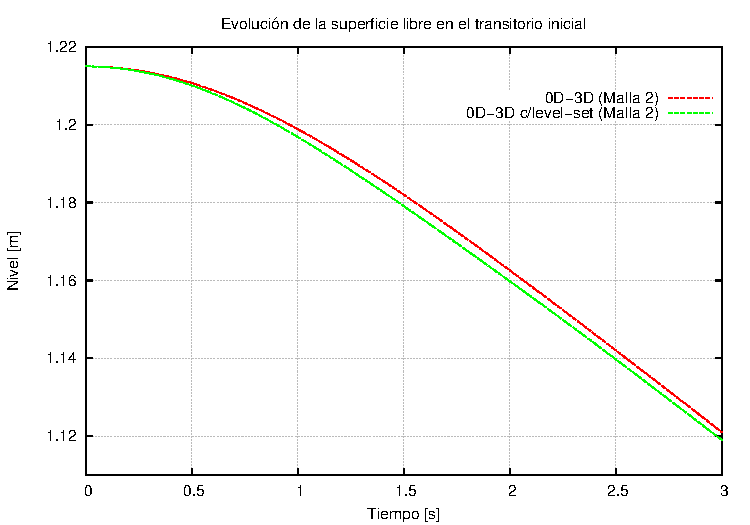
\includegraphics[scale = 1]{hvstlsZoom.pdf}
\caption[Evolución del nivel de líquido en el \textit{mockup} del tanque del reflector del reactor OPAL ante accionamiento del SSP]
{Evolución del nivel de líquido en el \textit{mockup} del tanque del reflector del reactor OPAL ante accionamiento del SSP durante el transitorio inicial.
  Se comparan la solución obtenida despreciando el gas en la cañería y la obtenida con transporte de superficie libre mediante la técnica de \textit{level-set}.}  
	\label{hvstls}
\end{figure}

En la Figura \ref{hvst} se compara la evolución obtenida de la superficie libre con los resultados anteriores,
y en la Figura \ref{hvstls} se compara la evolución durante el transitorio inicial.
Puede observarse que al modelar el transporte del gas la descarga se acelera durante el primer instante, debido a la menor pérdida de carga.
Sin embargo, este fenómeno no tiene mayor influencia.
La evolución posterior es similar a la obtenida sin el modelado de la superficie libre,
y por lo tanto la aproximación realizada inicialmente es conservativa, ya que considera una mayor pérdida de carga.

En la Figura \ref{evol-ls} se observa la evolución de la superficie libre en el arreglo de válvulas durante los primeros instantes de tiempo.

\begin{figure}[ht]
\begin{minipage}[t]{.48\textwidth}
\centering
\subfloat[t = 0 s]{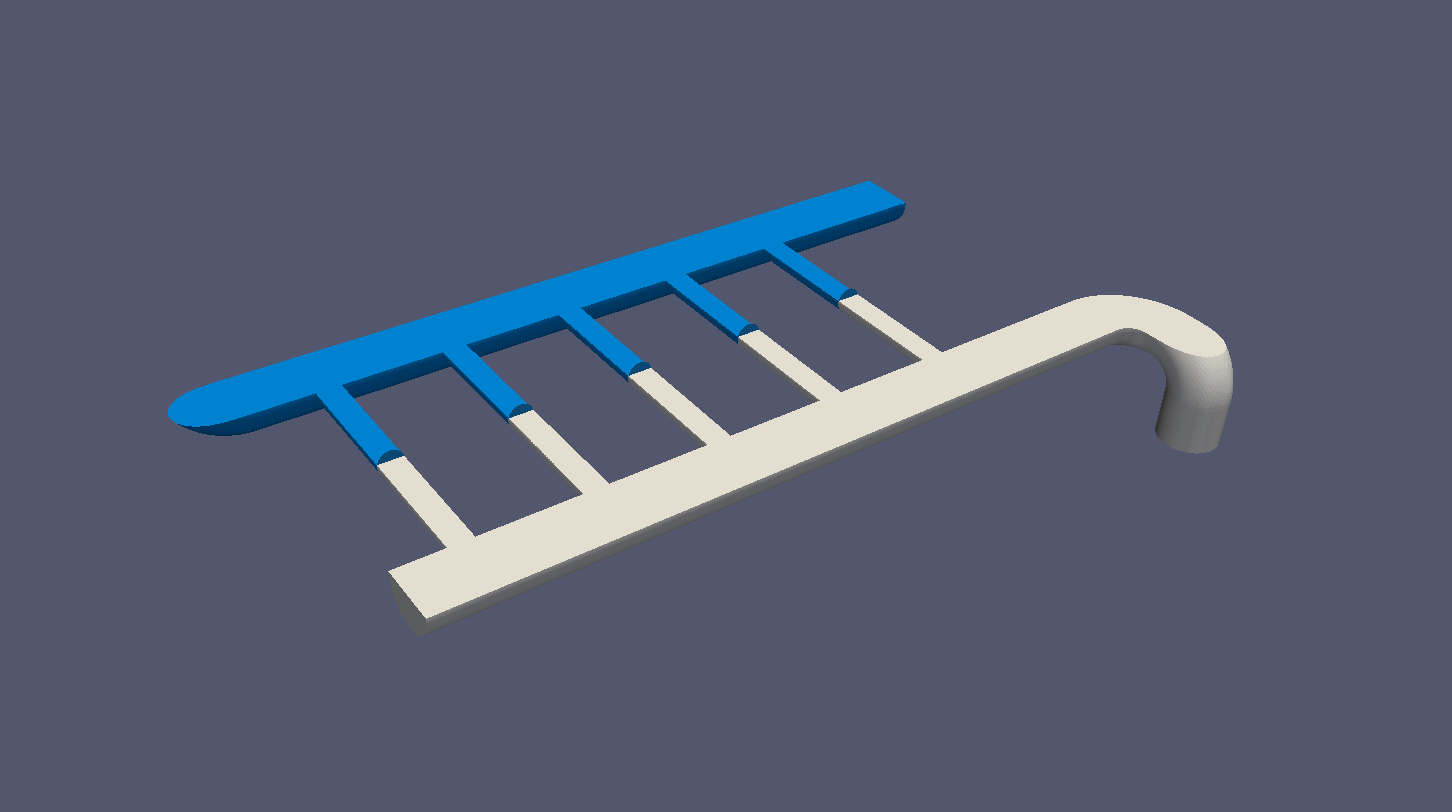
\includegraphics[scale=0.15]{0ms.png}}\\
\subfloat[t = 0.6 s]{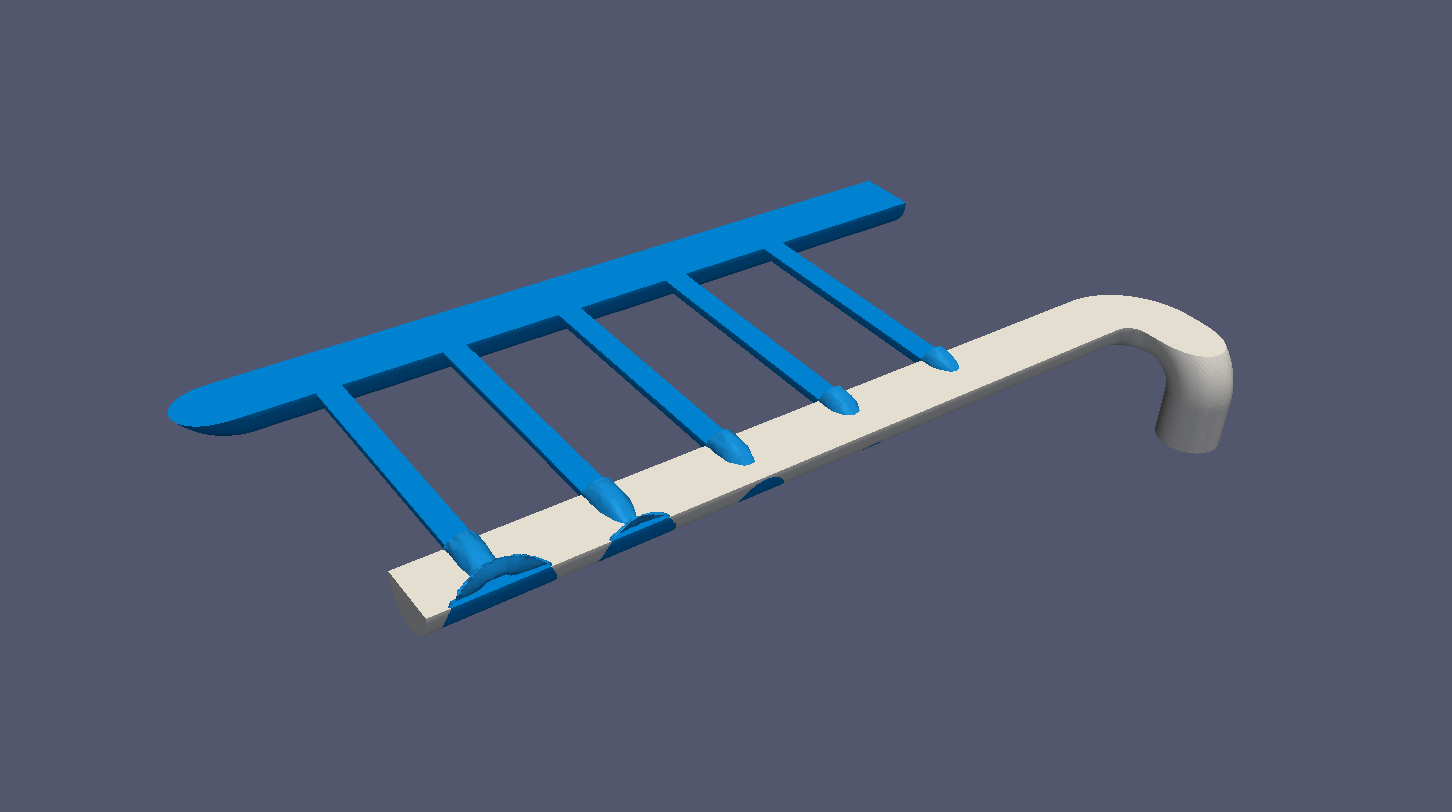
\includegraphics[scale=0.15]{600ms.png}}\\
\subfloat[t = 1.2 s]{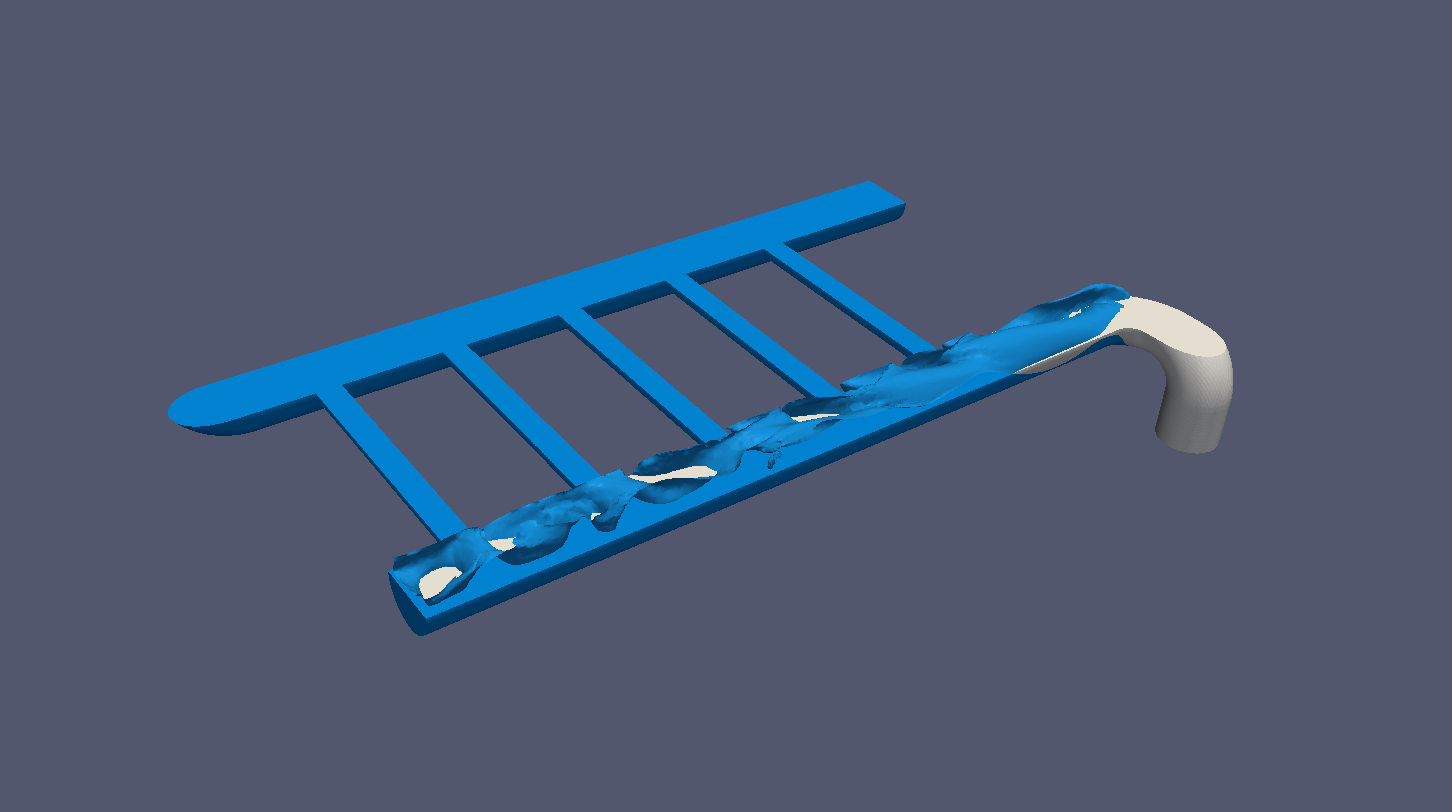
\includegraphics[scale=0.15]{1200ms.png}}
\end{minipage}\hfill
\begin{minipage}[t]{.48\textwidth}
\centering
\subfloat[t = 0.3 s]{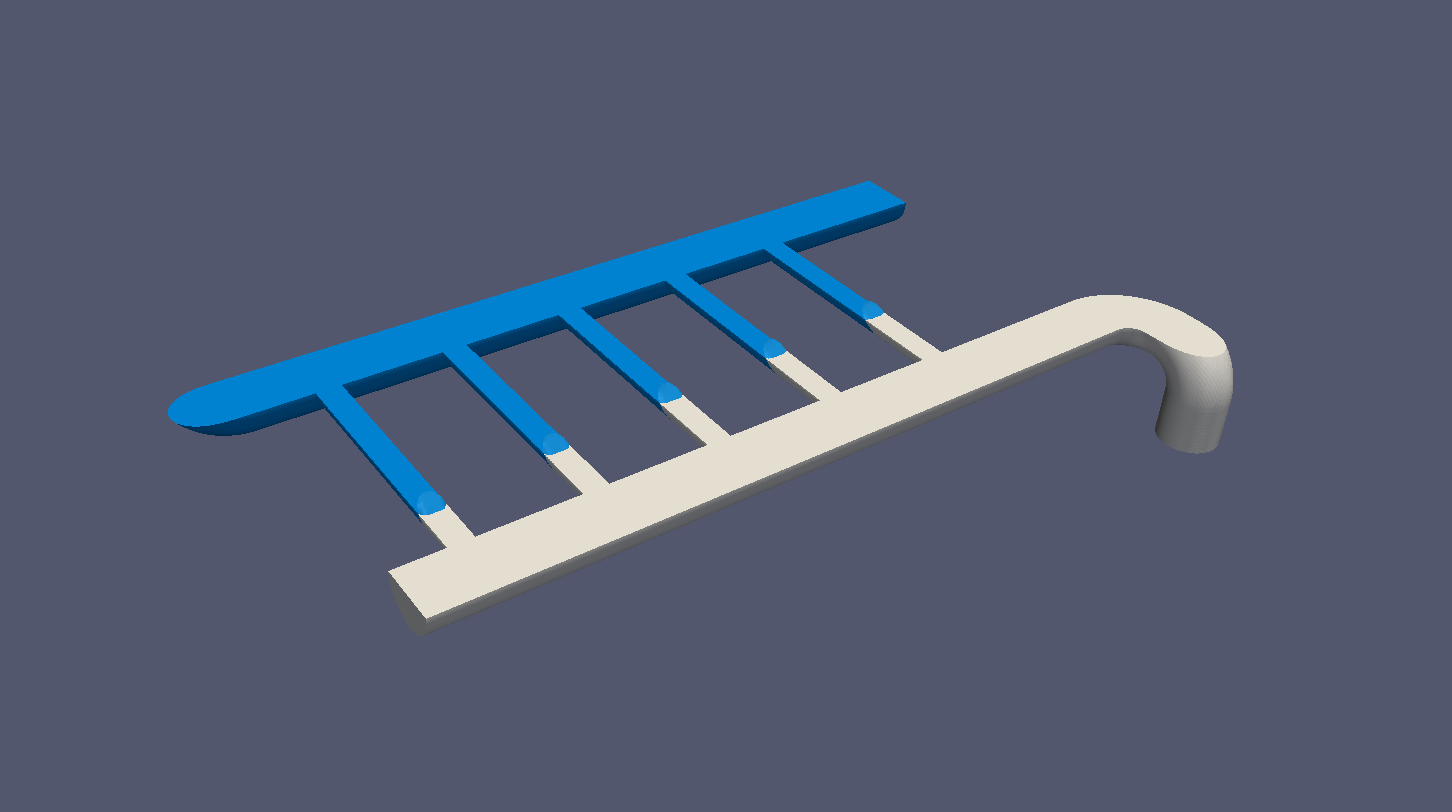
\includegraphics[scale=0.15]{300ms.png}}\\
\subfloat[t = 0.9 s]{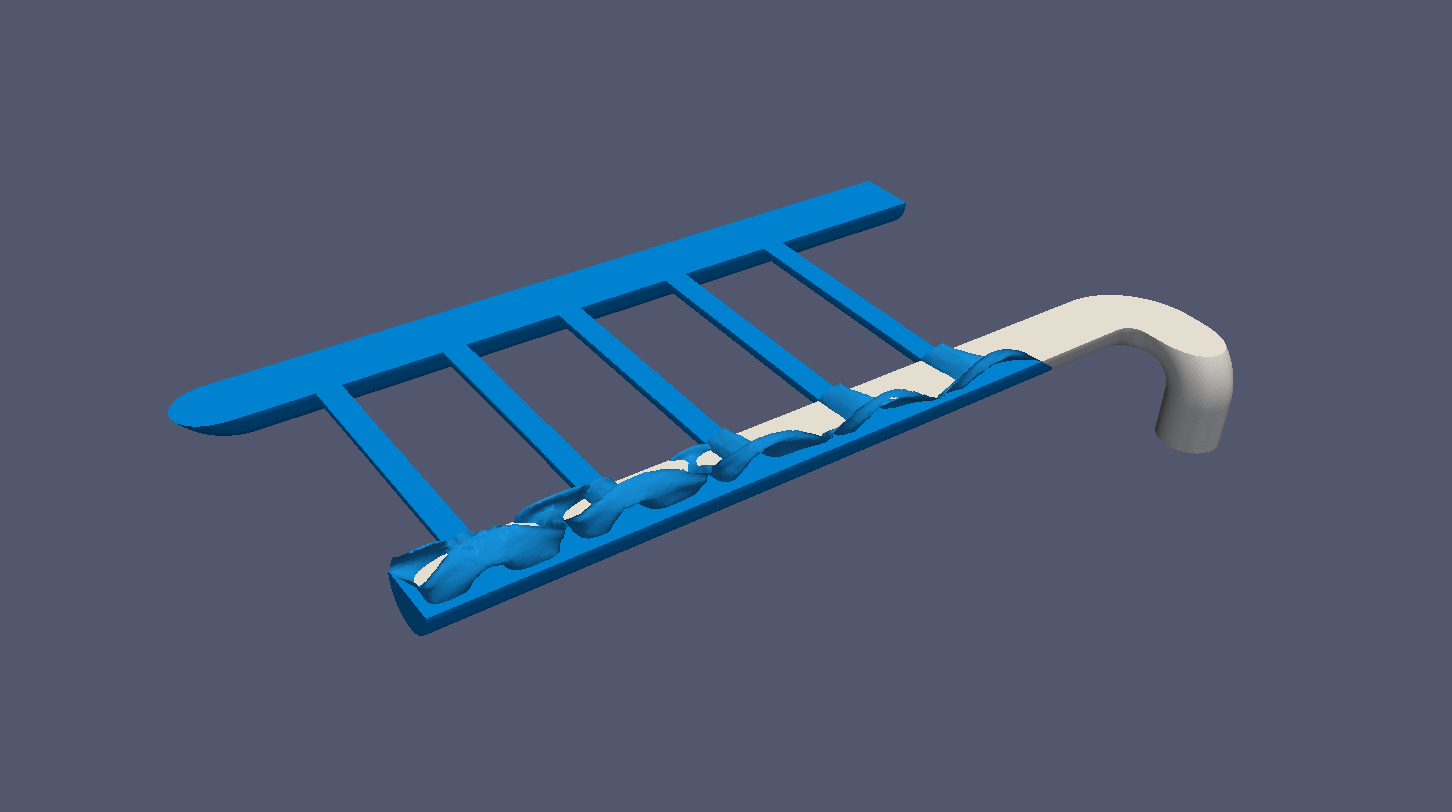
\includegraphics[scale=0.15]{900ms.png}}\\
\subfloat[t = 2.0 s]{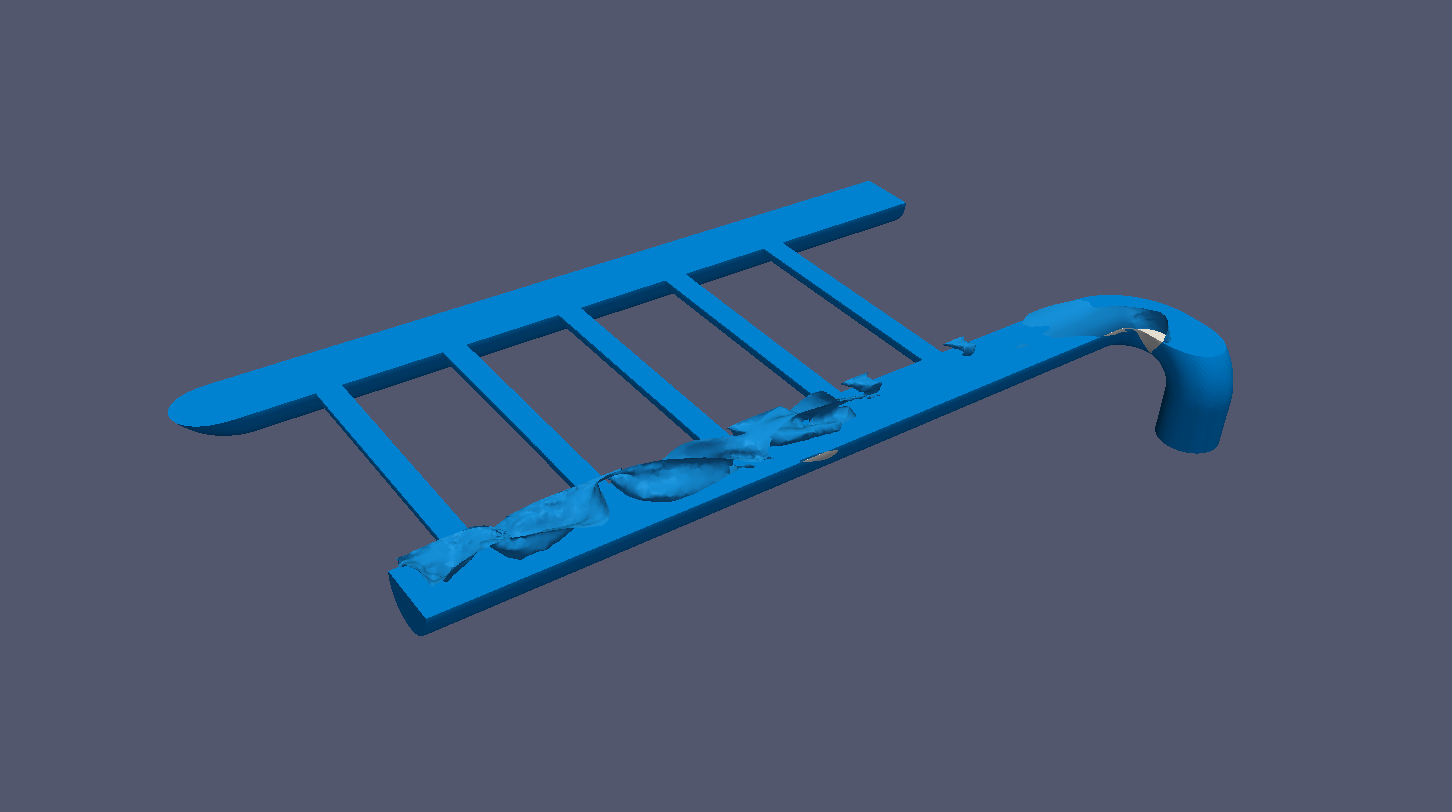
\includegraphics[scale=0.15]{2000ms.png}}
\end{minipage}
\caption[Transitorio inicial de la descarga del tanque a través del arreglo de válvulas del \textit{mockup} del reactor OPAL, con detalle de la evolución de la superficie libre]
{Transitorio inicial de la descarga del tanque a través del arreglo de válvulas, con falla simple en la última válvula
  (no se modela).
	El corte horizontal en la geometría permite observar el detalle de la evolución de la superficie libre.
  El líquido (azul) se encuentra inicialemente en condición estática rellenando las cañerías hasta la posición de las válvulas.
  Al otro lado el gas (blanco) rellena el resto de la red hidráulica.}  
\label{evol-ls}
\end{figure}

\subsection*{Conclusiones del análisis}
La herramienta de análisis de acoplamiento fuerte de subsistemas permite incorporar el estudio de la inercia fluídica en la red hidráulica de descarga.
Este estudio revela que los modelos que incluyen el fenómeno inercial del fluido en la red hidráulica del \textit{mockup} del SSP del OPAL predicen un retraso de la descarga en un máximo de un segundo 
respecto a los modelos que no lo incluyen.
Como la inclusión del efecto inercial modela una dinámica similar a la reportada experimentalmente durante el transitorio inicial y,
además, es conservativa en función del objetivo de estudio establecido, debería ser considerada en futuros análisis de seguridad.

\subsection*{Análisis de métodos de resolución del sistema de ecuaciones de residuos}

A fines de comparar la efectividad de diferentes métodos numéricos se realizaron distintos cálculos utilizando la malla más gruesa.
La Figura \ref{nonlinear_fevals} compara la cantidad de evaluaciones de funciones en función del paso temporal para diferentes métodos de resolución.

\begin{figure}[ht]
\centering
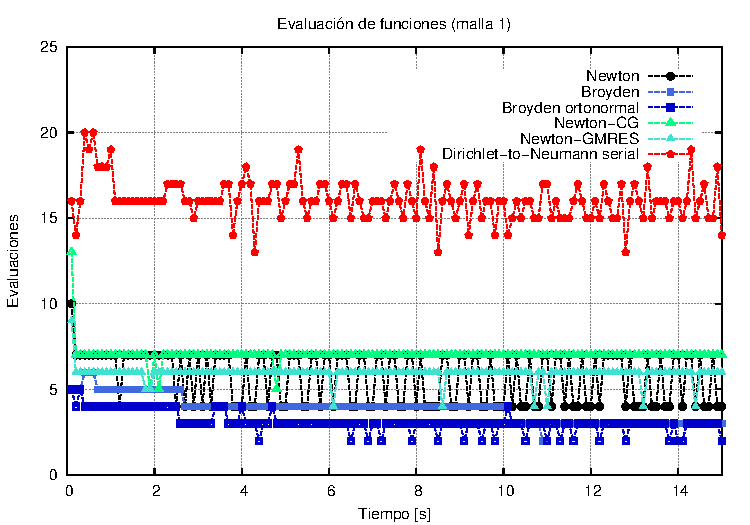
\includegraphics[scale = 1]{nonlinear_fevals.pdf}
\caption[Evaluación de diferentes métodos numéricos no lineales en el problema del vaciado del tanque reflector del \textit{mockup} del reactor OPAL]
{Evaluación de diferentes métodos numéricos en la resolución del sistema de ecuaciones de residuos resultante para el problema del vaciado del tanque reflector del \textit{mockup} del reactor OPAL.
El método explícito \textit{Dirichlet-to-Neumann} requiere excesiva cantidad de evaluaciones en cada paso de tiempo,
mientras que los métodos implícitos \textit{quasi-Newton} son los más eficientes.}
\label{nonlinear_fevals}
\end{figure}

El método explícito \textit{Dirichlet-to-Neumann} es el que mayor cantidad de evaluaciones consume, debido a que requiere una excesiva cantidad de iteraciones para converger.
Los métodos de tipo \textit{Newton-Krylov}: \textit{Newton-GMRES} y \textit{Newton-CG} (\textit{Newton-Gradientes Conjugados}) requieren baja cantidad de iteraciones, 
pero debido a la forma de resolución toman más evaluaciones que los métodos \textit{quasi-Newton}: \textit{Broyden} y \textit{Broyden ortonormal},
los cuales convergen con baja cantidad de iteraciones y de evaluaciones asociadas
(solo en el primer paso de cálculo involucran mayor cantidad de evaluaciones debido a que inicializan la matriz jacobiana por diferencias finitas).
El método de \textit{Newton-Raphson} toma tantas evaluaciones como los métodos \textit{Newton-Krylov},
sin embargo, estas evaluaciones están asociadas a muy baja cantidad de iteraciones,
ya que consume evaluaciones en la construcción de la matriz jacobiana.

En conclusión, al igual que en los resultados presentados en la sección \ref{3:mockup}, los métodos \textit{Broyden} y \textit{Broyden ortonormal} resultaron ser los más eficientes.
A fines de acelerar aún más el cálculo, se estudió la forma de optimizarlos.
Se ensayaron diferentes métodos para la propuesta de semillas del vector de incógnitas $\bar{x}_n$ y de la matriz $\mathbb{B}_n$ para cada paso temporal de resolución.
Hasta ahora las semillas para el primer paso temporal eran el vector de ceros $\bar{x}_1=\bar{0}$ y la matriz identidad $\mathbb{B}_1=\mathbb{I}$,
y las semillas para cualquier paso temporal próximo eran el vector $\bar{x}_{n-1}$ de la solución convergida en el paso previo,
y la matriz $\mathbb{B}_{n-1}$ de la última iteración correspondiente a ese paso.
Ahora el objetivo radica en intentar generar semillas que aceleren la convergencia.

Se propone utilizar un método de extrapolación, a partir de la información de los resultados que se van obteniendo en los sucesivos pasos.
La semillas para $\bar{x}_n$ y para $\mathbb{B}_n$ podrían tener órdenes de extrapolación $k_{\bar{x}}$ y $k_{\mathbb{B}}$ diferentes.
En el paso $n$, se van a utilizar los valores de los vectores $\bar{x}_i$, con $i  \in  \left \{ n-1-k_{\bar{x}}, n-1\right \}$,
y los valores de las matrices $\mathbb{B}_j$, con $j  \in  \left \{ n-1-k_{\mathbb{B}}, n-1\right \}$.
Estas extrapolaciones son válidas solo cuándo $n>k_{\bar{x}}+1$ y $n>k_{\mathbb{B}+1}$ respectivamente.

\begin{figure}[ht]
\centering
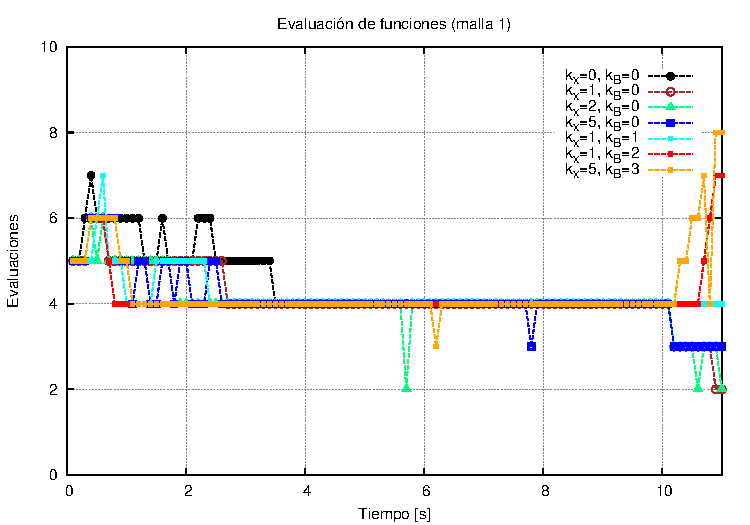
\includegraphics[scale = 1]{nonlinear_fevals_ex.pdf}
\caption[Eficiencia para diferentes esquemas de extrapolación en la generación de semillas]
{Eficiencia para diferentes esquemas de extrapolación en la generación de semillas para $\bar{x}_n$ y $\mathbb{B}_n$ en cada paso temporal.
$k_{\bar{x}}$ indica el órden de extrapolación para $\bar{x}_n$ y $k_{\mathbb{B}}$ indica el órden de extrapolación para $\mathbb{B}_n$ utilizado en cada esquema.
Los métodos con alto órden de extrapolación para $\mathbb{B}_n$ requieren menor cantidad de iteraciones para converger el cálculo en la primer etapa,
pero a su vez requieren excesivas iteraciones ante alguna perturbación en los resultados.
Los métodos con algún órden de extrapolación para $\bar{x}_n$ son más eficientes en estas instancias.}
\label{nonlinear_fevals_ex}
\end{figure}
La Figura \ref{nonlinear_fevals_ex} reporta la cantidad de evaluaciones de funciones requeridas para la convergencia en cada paso temporal,
jugando con diferentes órdenes de extrapolación para $\bar{x}_n$ y $\mathbb{B}_n$.
Las evaluaciones de funciones aquí están directamente relacionadas con las iteraciones necesarias para la convergencia,
ya que el método de \textit{Broyden} realiza una sola evaluación en cada iteración.
Al comienzo del cálculo todos los esquemas numéricos requieren excesivas iteraciones para converger,
y luego comienzan a converger con menor cantidad de iteraciones.
El cálculo con órden nulo de extrapolación para ambas variables es el que más tarda en bajar la cantidad de iteraciones.
Le siguen todos aquellos esquemas sin extrapolación para la matriz $\mathbb{B}_n$.
Los esquemas con $k_{\mathbb{B}}=3$ y $k_{\mathbb{B}}=5$ son los que más rápidamente bajan la cantidad de iteraciones,
por lo que se deduce que la extrapolación para la generación de semillas para $\mathbb{B}_n$ es altamente útil para arrancar el cálculo.
En etapas avanzadas la matriz $\mathbb{B}_n$ se estabiliza y comienza a converger a resultados similares en los sucesivos pasos.
Es decir, la tasa de cambio del vector solución $\bar{x}_n$ se vuelve aproximadamente constante (como puede observarse en la Figura \ref{qpvst}).
Ante una pequeño cambio, los esquemas de extrapolación para $\mathbb{B}_n$ amplifican esta perturbación y comienzan a generar malas semillas,
por lo que comienzan a requerir mayor cantidad de iteraciones para converger.
Este efecto puede observarse a partir de los $10s$ de cálculo.
Por el contrario, los esquemas con bajo órden de extrapolación para $\mathbb{B}_n$ y algún órden de extrapolación para $\bar{x}_n$ son más eficientes en esta etapa.
Aquí podría pensarse que los esquemas de extrapolación son inestables ante perturbaciones en $\mathbb{B}_n$, pero estables para perturbaciones en $\bar{x}_n$.

En base a estos resultados, se deduce que el esquema de generación de semillas idóneo
requiere órdenes de extrapolación $k_{\bar{x}}$ y $k_{\mathbb{B}}$ dependientes del tiempo,
comenzando con alto $k_{\mathbb{B}}$ y bajo $k_{\bar{x}}$, y tendiendo a $k_{\mathbb{B}}=0$ y alto $k_{\bar{x}}$ a medida que avanza el cálculo.

\section{Resolución de redes hidráulicas de múltiples componentes}
\label{3:redes}

\subsection*{Presentación del problema}
\label{3:redes-presentacion}

Con interés en conocer el comportamiento de la metodología de resolución
para problemas abordados mediante el Método de Descomposición Dijsunta de Dominios en sistemas con grandes cantidades de incógnitas,
se propuso analizar redes hidráulicas de múltiples componentes interconectados.
La idea es utilizar modelos sencillos que describan el comportamiento de cada componente particular para poder centrar el análisis solo en el estudio de convergencia
de resultados, analizando estados estacionarios.

\subsection*{Subsistemas de estudio}
\label{3:redes-subsistemas}

Se proponen sistemas de redes hidráulicas ramificadas divergentes.
Debido a la metodología de abordaje propuesta en el trabajo, las interfaces deben seleccionarse de forma que cada una de ellas solo conecte dos subdominios contiguos.
Por lo tanto, cada porción del sistema que comprende una ramificación es pensada como un subdominio diferente,
de modo que cada subdominio contenga tres interfaces de acoplamiento.
La Figura \ref{net16} esquematiza un modelo de estudio con 5 subsistemas acoplados.
Los parámetros geométricos de cada subsistema se sortean aleatoriamente entre valores típicos.
El fluido de trabajo es agua a temperatura y presión ambiente.

\begin{figure}[ht]
\centering{}
\begin{tikzpicture}

% Nodos
\node [label={\small $S_3$}] at (0em,0em) (n8) {};

\node [right of=n8, xshift=3em, yshift=-2em, align=center] (n13) {\small $v_{3,3}, \quad v_{5,1},$ \\ $P_{3,3}$ \quad $P_{5,1}$};
\node [right of=n13, xshift=3em, yshift=-2em, label={\small $S_5$}] (n14) {};
\node [right of=n14, xshift=2em, yshift=-2em] (n16) {\small $CB_{5,3}$};
\node [right of=n14, xshift=2em, yshift=2em] (n15) {\small $CB_{5,2}$};

\node [right of=n8, xshift=3em, yshift=2em, align=center] (n9) {\small $v_{3,2}, \quad v_{4,1},$ \\ $P_{3,2}$ \quad $P_{4,1}$};
\node [right of=n9, xshift=3em, yshift=0em, label={\small $S_4$}] (n10) {};
\node [right of=n10, xshift=2em, yshift=-2em] (n12) {\small $CB_{4,3}$};
\node [right of=n10, xshift=2em, yshift=2em] (n11) {\small $CB_{4,2}$};

\node [left of=n8, xshift=-3em, yshift=2em, align=center] (n7) {\small $v_{1,3}, \quad v_{3,1},$ \\ $P_{1,3}$ \quad $P_{3,1}$};
\node [left of=n7, xshift=-4em, yshift=3em, label={\small $S_1$}] (n2) {};
\node [left of=n2, xshift=-1em, yshift=-0em] (n1) {\small $CB_{1}$};

\node [right of=n2, xshift=4em, yshift=3em, align=center] (n3) {\small $v_{1,2}, \quad v_{2,1},$ \\ $P_{1,2}$ \quad $P_{2,1}$};
\node [right of=n3, xshift=3em, yshift=0em, label={\small $S_2$}] (n4) {};
\node [right of=n4, xshift=2em, yshift=2em] (n5) {\small $CB_{2,2}$};
\node [right of=n4, xshift=2em, yshift=-2em] (n6) {\small $CB_{2,3}$};

% Conexiones
\draw[|-] (n1.east) to [in=180, out=0] (n2.center);
\draw[-o] (n2.center) to[in=180, out=0] (n3.west);
\draw[-o] (n2.center) to[in=180, out=0] (n7.west);

\draw[o-] (n3.east) to[in=180, out=0] (n4.center);
\draw[-|] (n4.center) to[in=180, out=0] (n5.west);
\draw[-|] (n4.center) to[in=180, out=0] (n6.west);

\draw[o-] (n7.east) to[in=180, out=0] (n8.center);
\draw[-o] (n8.center) to[in=180, out=0] (n9.west);
\draw[-o] (n8.center) to[in=180, out=0] (n13.west);

\draw[o-] (n9.east) to[in=180, out=0] (n10.center);
\draw[-|] (n10.center) to[in=180, out=0] (n11.west);
\draw[-|] (n10.center) to[in=180, out=0] (n12.west);

\draw[o-] (n13.east) to[in=180, out=0] (n14.center);
\draw[-|] (n14.center) to[in=180, out=0] (n15.west);
\draw[-|] (n14.center) to[in=180, out=0] (n16.west);

\end{tikzpicture}
\caption[Descomposición disjunta de dominios en el modelado de redes hidráulicas]
{Descomposición disjunta de dominios en un modelo de red hidráulica con 16 incógnitas en las interfaces de acoplamiento.
La incógnita $v_{i,j}$ refiere a la velocidad media en el extremo $j$ del subsistema $i$.
La incógnita $P_{i,j}$ agrupa las presiones estática y dinámica medias en el extremo $j$ del subsistema $i$.
Las incógnitas pueden reducirse rápidamente a la mitad aplicando las relaciones de continuidad \ref{continuidad}.}
\label{net16}
\end{figure}

Cada subdominio es modelado con balances cero-dimensionales de conservación de masa y energía.
Las ecuaciones resultantes para un subsistema genérico que no contiene bordes del dominio original son las siguientes:
\begin{equation}
\left \{
\begin{array}{rcl}
\frac{p_1}{\rho} + \frac{{v_1}^2}{2} &=& \frac{p_2}{\rho} + \frac{{v_2}^2}{2} + gz_2 + \Delta u_{12} \\
\frac{p_1}{\rho} + \frac{{v_1}^2}{2} &=& \frac{p_3}{\rho} + \frac{{v_3}^2}{2} + gz_3 + \Delta u_{13} \\
A_1 v_1 &=& A_2 v_2 + A_3 v_3
\end{array}
\right .
\label{net-eq}
\end{equation}
donde los subíndices $1$, $2$ y $3$ refieren a diferentes extremos locales del contorno del subdominio,
$p_i$, $v_i$, $z_i$, y $A_i$ indican \textit{presión}, \textit{velocidad}, \textit{altura} y \textit{área} de la sección en el extremo $i$ respectivamente,
y $\Delta u_{ij}$ refiere a la diferencia de energía del flujo entre los exremos $i$ y $j$.
El extremo 1 siempre corresponde al izquierdo de cada subdominio, y las otros se numeran en forma horaria creciente.
Deben prestarse algunas consideraciones extras en las ecuaciones para los subsistemas que requieren condiciones $CB_{k,l}$ sobre extremos que pertenecían al borde original del sistema completo,
donde $k$ indica el subsistema y $l$ el extremo local.

Los términos de presión estática $\frac{p_i}{\rho}$ y presión dinámica $\frac{{v_i}^2}{2}$ para el extremo $i$ pueden agruparse en una única incógnita $P_i$ para simplificar el cálculo:

\begin{equation}
P_i = \frac{p_i}{\rho} + \frac{{v_i}^2}{2}
\label{p-eyd}
\end{equation}

El término $\Delta u_{ij}$ puede aproximarse mediante una función de pérdida de carga como \cite{white}:
\begin{equation}
\Delta u_{ij} = \frac{{v_i}^2}{2} \left ( \frac{f_{D_i} L_{i}}{D_i} + \sum_t K_{i,t} \right ) + \frac{{v_j}^2}{2} \left ( \frac{f_{D_j} L_{j}}{D_j} + \sum_t K_{j,t} \right )
\label{du}
\end{equation}
En esta ecuación, el primer término está modelando la pérdida de carga total entre el extremo $i$ y el nodo de divergencia,
y el segundo extremo modela la pérdida de carga total entre este nodo y el extremo $j$.
Las variables $D_i$ y $L_i$ corresponden al \textit{diámetro} y a la \textit{longitud} de la cañería desde el extremo $i$ hasta el nodo de divergencia,
$f_{D_i}$ corresponde al \textit{factor de Darcy} del flujo en esa porción
y $K_{i,t}$ corresponde al \textit{factor de pérdida de carga concentrada t} de cualquier componente hidráulico presente lo largo de algún punto de esa porción de cañería.
Bajo algunas modificaciones sería posible incorporar cambios en las secciones a lo largo de estas porciones, pero no se realizó por simplicidad.

Considerando que el flujo corre por la red hidráulica en régimen laminar, el \textit{factor de Darcy} $f_{D_i}$ puede modelarse como \cite{white}:
\begin{equation}
f_{D_{{i},lam}} = \frac{64}{Re_{D_i}}
\label{f-lam}
\end{equation}
donde $Re_{D_i}=\frac{\rho v_i D_i} {\mu_i}$, siendo $\mu$ la viscocidad dinámica del fluido.
Bajo esta aproximación, la ecuación \ref{du} queda lineal en $v_i$ y en $v_j$ para aquellos subsistemas en los que pudiera despreciarse la pérdida de carga concentrada:
\begin{equation}
\Delta u_{ij,lam} = \frac{{v_i}}{2} \left ( \frac{64 \mu L_{i}}{\rho {D_i}^{2}} \right ) + \frac{{v_j}}{2} \left ( \frac{64 \mu L_{j}}{\rho {D_j}^{2}} \right )
\label{du}
\end{equation}


\subsection*{Estrategia de resolución}
\label{resolucion-net}

Conforme al esquema de resolución descripto en la sección \ref{1:abordaje},
es necesario definir una estrategia para las condiciones de borde en las interfaces de acoplamiento de cada subsistema.
La estrategia propuesta es establecer condiciones de tipo \textit{Dirichlet} sobre las interfaces ubicadas a la izquierda de cada subdominio (fijando $v$)
y condiciones de tipo \textit{Neumann} sobre las interfaces ubicadas a la derecha (fijando $P$).
Considerando las ecuaciones de continuidad \ref{continuidad} se seleccionan una serie de ecuaciones modelos \ref{ecuaciones-modelos}
a partir de las relaciones \ref{net-eq} de manera que cada subproblema quede bien planteado.
En cada interfaz de acoplamiento $j$ de cada subsistema $i$ queda definida una ecuación de residuo:

\begin{equation}
(R_{p,Q})_{i}^{j}=0 \\
\end{equation}
donde $R_{p,Q}$ es la diferencia entre el valor de la variable calculada en la interfaz $j$ del subsistema $i$ y el valor de la semilla correspondiente.

Las ecuaciones de cada subsistema son resueltas mediante funciones escritas en \texttt{Octave}.
En este caso el acoplamiento de funciones se da a través de una función \textit{maestra} también escrita en \texttt{Octave}.

\subsection*{Redes hidráulicas con regímenes de flujo laminar}
\label{laminar}

En la Figura \ref{net_linear} (a) se pueden observar la cantidad de iteraciones requeridas por diferentes métodos para la convergencia de resultados
en sistemas hidráulicos laminares sin pérdidas de carga concentrada,
variando la cantidad de subsistemas acoplados.
La cantidad de incógnitas en el eje $x$ corresponde a la simplificación obtenida tras aplicar las ecuaciones de continuidad \ref{continuidad}.

\begin{figure}[ht]
	\begin{minipage}{0.5\linewidth}
		\centering
		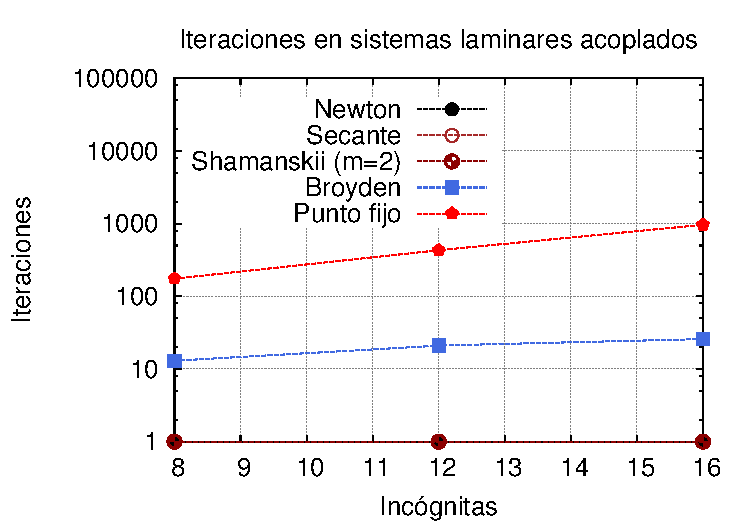
\includegraphics[scale=0.55]{net_linear_its.pdf}
	\end{minipage}
	\begin{minipage}{0.5\linewidth}
		\centering
		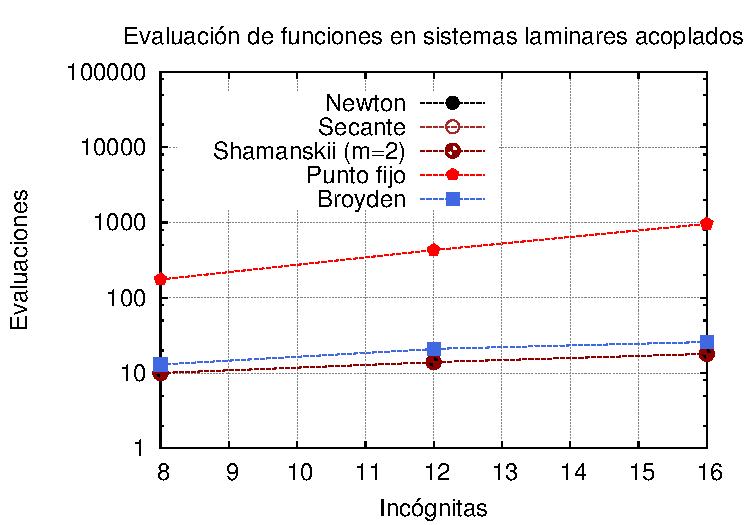
\includegraphics[scale=0.55]{net_linear_fevals.pdf}
	\end{minipage}
	\caption[Comparación de diferentes métodos numéricos para la resolución de sistemas de redes hidráulicas]
  {Comparación de diferentes métodos numéricos para la resolución de sistemas de redes hidráulicas:
  (a) iteraciones requeridas y (b) evaluaciones de funciones requeridas.}
  \label{net_linear}
\end{figure}

En la figura se observa que el método del punto fijo requiere excesiva cantidad de iteraciones.
Las mismas ascienden hasta 1000 para sistemas con 16 incógnitas reducidas,
pero este valor puede variar dependiendo de las semillas iniciales y de los parámetros del sistema.
El método de \textit{Broyden} requiere decenas de iteraciones para cada sistema.
El método de \textit{Newton-Raphson}, el método de la \textit{secante}
y el método de \textit{Shamanskii} de tipo $m$=2
requieren solo una iteración, debido a que los sistemas de cálculo son lineales
(las tres curvas se encuentran superpuestas).
Sin embargo, el parámetro de comparación de interés es la cantidad total de evaluaciones que requiere cada método.
En la Figura \ref{net_linear} (b) se observa que la ventaja obtenida por los métodos que construyen la matriz jacobiana es despreciable frente al método de \textit{Broyden}.

Debido a que los métodos \textit{quasi-Newton} han presentado elevada confiabilidad en la resolución de sistemas acoplados a lo largo de todo el trabajo,
se investigaron formulaciones alternativas al método de \textit{Broyden},
y en la Figura \ref{net_linear_its_broy} se reportan los resultados.

\begin{figure}[ht]
\centering
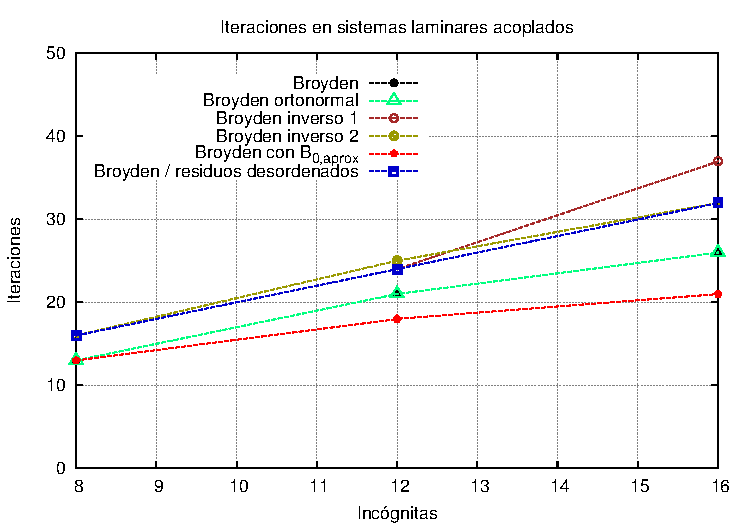
\includegraphics[scale = 1]{net_linear_its_broy.pdf}
\caption[Comparación de diferentes esquemas de \textit{Broyden} para la resolución de sistemas de redes hidráulicas con regímenes de flujo laminar]
{Comparación de diferentes esquemas de \textit{Broyden} para la resolución de sistemas de redes hidráulicas con regímenes de flujo laminar.}
	\label{net_linear_its_broy}
\end{figure}

Además del método \textit{Broyden ortonormal}, que en este estudio se comporta con igual eficiencia que el método de \textit{Broyden} (ambas curvas se solapan),
existen formulaciones que aproximan directamente la inversa de la matriz jacobiana (\textit{Broyden inverso 1} y \textit{Broyden inverso 2}).
Estos métodos se conocen en la bibliografía como \textit{bad Broyden update} (mala actualización de Broyden) \cite{griewank} y en la figura puede verse que tienen eficiencia inferior.

El método de \textit{Broyden} se utilizó también mejorando la semilla inicial para la matriz $\mathbb{B}_n$.
En los otros esquemas reportados se utiliza la matriz identidad,
pero aquí se reemplazó por una matriz con \textit{unos} en los elementos que corresponden a posiciones llenas de la matriz jacobiana original,
y \textit{ceros} en el resto de los elementos.
Este llenado es sencillo de implementar ya que simplemente depende de las relaciones de dependecia de las residuos y las incógnitas, que \textit{a priori} son conocidas.
Con esta implementación puede observarse en la curva de \textit{Broyden} con $\mathbb{B}_{0,aprox}$ que la convergencia mejora a medida que la cantidad de incógnitas aumenta.
Una mejor semilla para la matriz $\mathbb{B}_{0}$ hubiera podido generarse con un cálculo de diferencias finitas,
similar al que se venía utilizando para inicializar las matrices en las aplicaciones analizadas en \ref{3:ff} y \ref{3:mockup}.
En este caso los resultados hubieran coincidido con los resultados del método de la secante, que efectúa el cálculo aproximado de $\mathbb{J}$ y luego converge en una sola iteración.

Comúnmente las incógnitas tienen una numeración global, conforme al orden en el que se construyen las columnas de la matriz jacobiana
(cada columna representa la derivada del vector residuo respecto de alguna incógnita).
De ser posible, los residuos suelen ordenarse de forma tal que el residuo $i$ compute la diferencia entre el valor calculado y el valor \textit{guess} para la incógnita $i$.
En estos casos utilizar la matriz identidada como semilla para $\mathbb{B}_{0}$ es una buena propuesta.
La curva \textit{Broyden / residuos desordenados} corresponde a un esquema en el que el residuo $i$ se corresponde con alguna incógnita $j$ distinta de $i$.
Utilizar la matriz identidad como semilla para $\mathbb{B}_n$ es una mala propuesta en este caso,
ya que para cada fila $i$, el \textit{uno} debería ubicarse en la posición $j$.
Esto genera mayor dificultad para la convergencia.
Por lo tanto puede comprenderse que la diferencia entre las curvas \textit{azul} y \textit{roja} (que representan los resultados para el mismo método de \textit{Broyden})
depende exclusivamente de una elección inteligente en la forma de proponer la semilla para la matriz $\mathbb{B}_n$.
Esta diferencia asciende a 10 iteraciones en un sistema con 16 incógnitas reducidas.

\subsection*{Redes hidráulicas con regímenes de flujo turbulento}
\label{turbulent}

Habiendo investigado sistemas de redes hidráulicas con regímenes de flujo laminar,
el siguiente paso de estudio consiste en analizar sistemas de redes hidráulicas con regímenes de flujo turbulento.
En estos modelos se utiliza directamente la ecuación \ref{du} para representar la pérdida de carga entre dos extremos de un dado subdominio,
por lo que el sistema de ecuaciones global ahora es un sistema de ecuaciones no lineales.
Aquí los métodos estudiados en el apartado anterior se comportan de forma diferente.
El método de \textit{Newton-Raphson} ya no converge en una única iteración como lo hace en sistemas lineales.
La Figura \ref{net_nonLinear_fevals} detalla la cantidad de evaluaciones de funciones requerida por distintos métodos
para la convergencia de los resultados en sistemas con diferente cantidad de incógnitas reducidas.

\begin{figure}[ht]
\centering
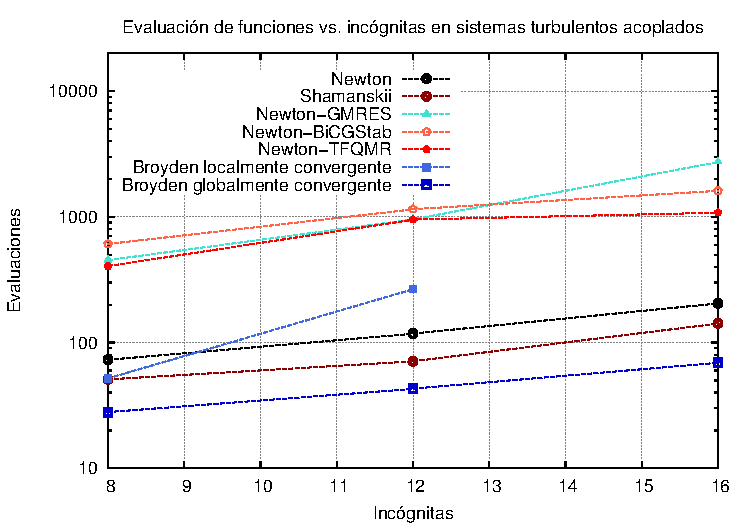
\includegraphics[scale = 1]{net_nonLinear_fevals.pdf}
\caption[Comparación de diferentes métodos numéricos para la resolución de sistemas de redes hidráulicas con regímenes de flujo turbulento]
{Comparación de diferentes métodos numéricos para la resolución de sistemas de redes hidráulicas con regímenes de flujo turbulento.}  
\label{net_nonLinear_fevals}
\end{figure}

El método explícito del punto fijo diverge en todos los sitemas analizados y por lo tanto no aparece en la gráfica.
Los métodos implícitos estudiados incluyen \textit{line searching}.
Los métodos \textit{Newton-Krylov} toman demasiadas evaluaciones para converger.
Los métodos de \textit{Newton-Raphson} y \textit{Shamanskii} tienen buena convergencia.
De estos dos el último presenta mayor ventaja ya que elude el cálculo de la matriz jacobiana en iteraciones contiguas.
El método que mejor se comporta es el método de \textit{Broyden} (globalmente convergente).
El método de \textit{Broyden local}, el único que no incluye \textit{line searching},
solo se comporta bien a baja cantidad de incógnitas, y cuando la cantidad de incógnitas es elevada diverge.

\section{Extensión a problemas acoplados en modelos de núcleo}
\label{3:extension-nucleo}

\subsection*{Estrategia de acoplamiento extendida}
\label{3:strategy-extended}

Si bien la estrategia de resolución presentada en el \hyperlink{chapter.2}{Capítulo 2}
corresponde a un equema para resolver problemas que han sido formulados mediante el Método de Descomposición Disjunta de Dominios,
el sistema de ecuaciones acoplado a resolver podría provenir de otras formulaciones,
y también ser abordados mediante la misma estrategia.
Es decir, la herramienta de acoplamiento puede ser utilizada para resolver cualquier tipo de sistemas de ecuaciones acopladas,
siempre que existan diferentes códigos que se encarguen de resolver parcialmente algunas de ellas.

A continuación se propone un modelo simplificado para el análisis de la dinámica de núcleo de un reactor nuclear.
En los dos últimos apartados se presentan ejemplos de acoplamiento neutrónico-termohidráulico utilizando este modelo.

\subsection*{Presentación del problema}
\label{3:neut-th}

La distribución espacial de la potencia generada en el núcleo de un reactor nuclear
depende de diversos factores, como la posición de barras de control, combustibles y demás materiales,
y de parámetros físicos como la temperatura del combustible, la temperatura del refrigerante o la fracción de vacío.
Los modelos neutrónicos que se utilizan para capturar esta dependencia modelan todos estos factores simplemente a través de una disposición espacial de secciones eficaces.
La distribución espacial de potencia, a su vez, genera modificaciones sobre las secciones eficaces,
ya sea debido a que está actuando como una fuente de energía, modificando temperaturas y densidades de combustibles, refrigerantes y demás materiales,
o debido al movimiento futuro requerido de materiales,
como por ejemplo, movimiento de barras de control necesarios para buscar perfiles de potencia planos, o recambio de combustibles por pérdida de criticidad.
Además, en la evolución temporal, el quemado de combustible genera alteraciones en la concentración de elementos existentes y aparición de nuevos elementos,
que también modifican las secciones eficaces.

La dinámica del núcleo de un reactor nuclear acopla fuertemente múltiples fenómenos, y cualquier modelo que se utilice para estudiarla debe abordar el acoplamiento mediante alguna estrategia.
En general, los códigos de cálculo utilizados en el área nuclear están validados para resolver solo alguno de estos fenómenos,
por lo que suele requerirse un acoplamiento entre ellos para resolver la dinámica completa.
Comúnmente este acoplamiento se resuelve mediante iteraciones explícitas de tipo \textit{Picard} dentro de cada paso de tiempo.

En esta sección se propone un modelo simplificado para el análisis de la dinámica de núcleo de un reactor nuclear durante un ciclo de quemado de elementos combustibles,
considerando solo los fenómenos neutrónico y termohidráulico.

\subsection*{Subsistemas de estudio}
\label{3:subsistemas-nt}

El cálculo de núcleo se efectúa mediante un modelo de difusión estacionario
\footnote{Al modelar un flujo neutrónico estacionario en realidad se está calculando el flujo en un reactor crítico asociado,
por lo que la distribución de potencia hallada solo es válida si el $k_{eff}$ calculado es igual a 1.
En caso contrario, debe repetirse el cálculo considerando otra distribución de secciones eficaces
(por ejemplo, moviendo barras de control).
} \cite{henry}:

\begin{equation}
\Delta \bar{\phi} = \frac{1}{k_{eff}}\Sigma \bar{\phi}
\label{eq-nucleo}
\end{equation}
donde $\bar{\phi}$ es una función vectorial con el valor del flujo neutrónico en cada punto del espacio para diferentes grupos de energía,
$\Sigma$ es la matriz de secciones eficaces asociada a diferentes reacciones para diferentes grupos de energía,
y $k_{eff}$ es el factor de criticidad del reactor.
En el modelo propuesto las secciones eficaces dependen de la densidad del refrigerante $N_{ref}$, de la temperatura del refrigerante $T_{ref}$, de la temperatura del combustible $T_{comb}$, 
y del valor histórico de quemado $B$ del material \cite{lamarsh},
para cada punto espacial y cada grupo de energía, de modo que:

\begin{equation}
\Sigma = \Sigma \left ( N_{ref}, T_{ref}, T_{comb} \right )
\label{eq-sigma}
\end{equation}

La ecuación \ref{eq-nucleo} requiere condiciones de borde en el contorno del dominio de cálculo.
En el primer ejemplo analizado se utilizan condiciones de borde homogéneas\footnote{
Imponer un flujo $\bar{phi}$ nulo en el contorno del dominio implica utilizar la hipótesis de que el flujo se hace nulo a alguna distancia del borde (en la \textit{distancia extrapolada} \cite{lamarsh}),
y asumir al mismo tiempo que esta distancia es despreciable, para de esta forma no extender el dominio de cálculo.
} sobre $\phi$.
En el segundo ejemplo analizado se imponen condiciones de flujo entrante nulo.
Éstas se modelan mediante un artificio de absorción total de los neutrones salientes, extendiendo la malla del cálculo.

Una vez obtenido el flujo neutrónico $\phi$,
la distribución de potencia $P$ puede calcularse a partir del ritmo de reacciones de fisión \cite{lamarsh}:

\begin{equation}
P = \int_{vol} E_{fis,i} \Sigma_{fis,i} \phi_{i}
\label{power}
\end{equation}
donde $E_{fis,i}$ es la energía liberada por fisiones ocurridas en el rango de energía $i$,
$\Sigma_{fis,i}$ es la sección eficaz de fisión condensada en el grupo de energía $i$ y
$\phi_{i}$ es la componente del flujo neutrónico también dondensada en el grupo de energía $i$.
La distribución de potencia ${P}$ hallada es utilizada como fuente de energía en los cálculos acoplados de transferencia de energía.

Los fenómenos hidrodinámicos y de transferencia de calor se modelan con ecuaciones uni-dimensionales y transitorias.
La transferencia de calor a través de las estructuras de combustibles se modela con la siguiente ecuación diferencial:

\begin{equation}
\rho \frac{\partial T_{comb}}{\partial t} = \nabla \left ( k \nabla T \right )  + S
\label{relap-calor}
\end{equation}
donde $\rho$ es la densidad del medio difusivo,
$T_{comb}$ es la temperatura del combustible,
$k$ es el coeficiente de conductividad térmica y
$S$ es la fuente interna de energía.
Este último término es el que tiene la información de la distribución de potencia generada en el núcleo del reactor.
El modelo se completa con condiciones de borde adecuadas.
El refrigerante fluye alrededor de las estructuras con temperatura media $T_{sk}$ y la energía transferida entre ambos se da por convección:

\begin{equation}
-k \frac{\partial T_{comb}}{\partial n} = h \left ( T - T_{sk} \right )
\label{relap-conveccion}
\end{equation}
donde $h$ es el coeficiente de transferencia de calor que debe obtenerse a partir de algún modelo adecuado para el régimen de flujo,
y $n$ es la dirección normal al borde del dominio de cálculo de $T_{comb}$.

El modelo hidrodinámico del comportamiento del refrigerante considera una mezcla del fluido en fases líquida y gaseosa.
Las ecuaciones básicas diferenciales de este modelo son seis \cite{manual-relap-modelos}.
Las primeras dos son las ecuaciones de continuidad en cada fase:

\begin{equation}
\left \{
\begin{array}{r}
\frac{\partial} {\partial t} \alpha_g \rho_g + \frac{1}{A} \frac{\partial}{\partial x} \left (\alpha_g \rho_g v_g A \right ) = \Gamma_g \\
\frac{\partial} {\partial t} \alpha_f \rho_f + \frac{1}{A} \frac{\partial}{\partial x} \left (\alpha_f \rho_f v_f A \right ) = \Gamma_f
\end{array}
\right .
\label{relap-masa}
\end{equation}
donde los subíndices $g$ y $f$ refieren a las fases gaseosa y líquida respectivamente,
$x$ es la dirección del flujo, normal a la sección de área $A$,
$\alpha_i$ refiere a la fracción parcial de área que la fase $i$ ocupa en $A$,
$\rho_i$ es la densidad del fluido en la fase $i$,
$v_i$ es la velocidad en la dirección $x$ del fluido en la fase $i$, promediada en la sección y
$\Gamma_i$ es un término de producción fluídica en la fase $i$.
Notar que este por continuidad, $\Gamma_g = -\Gamma_f$.

Las siguientes dos ecuaciones son las ecuaciones de momento de cada fase:

\begin{equation}
\left \{
\begin{array}{r}
\alpha_g \rho_g A \frac{\partial v_g}{\partial t} + \frac{1}{2} \alpha_g \rho_g A \frac{\partial v_g^2}{\partial x} = 
- \alpha_g A \frac{\partial P}{\partial x} + \alpha_g \rho_g B_x A - \left( \alpha_g \rho_g A \right) FWG \left (v_g \right) \\
+ \Gamma_g A \left( v_{gI} - v_g \right ) - \left ( \alpha_g \rho_g A \right ) FIG \left( v_g - v_f \right) \\
-C\alpha_g\alpha_f\rho_mA \left [ \frac{\partial \left( v_g - v_f \right)}{\partial t} + v_f \frac{\partial v_g}{\partial x} - v_g \frac{\partial v_f}{\partial x} \right ] \\

\alpha_f \rho_f A \frac{\partial v_f}{\partial t} + \frac{1}{2} \alpha_f \rho_f A \frac{\partial v_f^2}{\partial x} = 
- \alpha_f A \frac{\partial P}{\partial x} + \alpha_f \rho_f B_x A - \left( \alpha_f \rho_f A \right) FWF \left (v_f \right) \\
- \Gamma_g A \left( v_{fI} - v_f \right ) - \left ( \alpha_f \rho_f A \right ) FIF \left( v_f - v_g \right) \\
-C\alpha_f\alpha_g\rho_mA \left [ \frac{\partial \left( v_f - v_g \right)}{\partial t} + v_g \frac{\partial v_f}{\partial x} - v_f \frac{\partial v_g}{\partial x} \right ] \\
\end{array}
\right .
\label{relap-momento}
\end{equation}
La primera ecuación corresponde a la fase gaseosa y la segunda corresponde a la fase líquida.
Las ecuaciones son complejas y pueden analizarse separando los términos.
En cualquiera de ambas, los términos del lado izquierdo representan el transporte de momento.
Los términos de la derecha representan los agentes que generan el cambio de momento.
El primer término representa el cambio debido al gradiente de presión $P$.
El segundo término, debido a las fuerzas de volúmen $B_x$.
El tercero, debido a la fuerza de fricción en la pared con coeficientes $FWG$ en la fase gaseosa y $FWF$ en la fase líquida.
El cuarto término representa el momento transferido por intercambio de masa en la interfaz con velocidad $v_{gI}$ o $v_{fI}$.
El quinto término representa el cambio de momento debido a la fricción \textit{drag} interfacial,
cuyos coeficientes $FIG$ y $FIF$ dependen del modelo que se use, conforme al régimen de flujo.
El último término representa una fuerza dada por una masa virtual,
debido a la aceleración relativa entre las fases.
El coeficiente $C$ dependen del modelo que se utilice según el régimen de flujo.

Las últimas dos ecuaciones hidrodinámicas son las ecuaciones de conservación de energía $U_i$ para cada fase.
Considerando algunas simplificaciones \cite{manual-relap-modelos}, las ecuaciones son las siguientes:

\begin{equation}
\left \{
\begin{array}{r}
\frac{\partial}{\partial t} \left( \alpha_g \rho_g U_g\right) + \frac{1}{A} \frac{\partial}{\partial x} \left ( \alpha_g \rho_g U_g v_g A \right ) = 
-P \frac{\partial \alpha_g}{\partial t} - \frac{P}{A} \frac{\partial}{\partial x} \left( \alpha_g v_g A \right ) \\
+ Q_{wg} + Q_{ig} + \Gamma_{ig}h^*_g + \Gamma_w {h}'_g + DISS_g \\

\frac{\partial}{\partial t} \left( \alpha_f \rho_f U_f\right) + \frac{1}{A} \frac{\partial}{\partial x} \left ( \alpha_f \rho_f U_f v_f A \right ) = 
-P \frac{\partial \alpha_f}{\partial t} - \frac{P}{A} \frac{\partial}{\partial x} \left( \alpha_f v_f A \right ) \\
+ Q_{wf} + Q_{if} - \Gamma_{ig}h^*_f + \Gamma_w {h}'_f + DISS_f
\end{array}
\right .
\label{relap-energia}
\end{equation}
La primera ecuación corresponde a la fase gaseosa y la segunda corresponde a la fase líquida.
Los términos de la izquierda representan el transporte de energía en cada fase.
Los dos primeros términos de la derecha representan trabajo por cambio de fase.
El tercer término de la derecha en cada ecuación representa la transferencia de calor con las paredes de las estructuras,
y son los términos que acoplan la dinámica fluídica a la distribución de temperatura en los combustibles, (ver ecuación \ref{relap-conveccion}.
El cuarto término en cada ecuación representa la transferencia de calor en la interfaz entre las fases.
El quinto término en cada ecuación representa la transferencia de calor debido al cambio de fase en la interfaz.
El cambio de masa $\Gamma_{ij}$ en la interfaz $i$ y la fase $j$ tiene asociado una entalpía de fase $h^*_j$.
Los anteúltimos términos representan la transferencia de calor debido al cambio de fase por contacto con la pared.
El cambio de masa $\Gamma_{w}$ en la pared $w$ y la fase $j$ tiene asociado una entalpía de fase ${h}'_j$.
Finalmente, los últimos términos $DISS_i$ representan disipación viscosa en la fase $i$ por fricción en la pared.

En las ecuaciones \ref{relap-momento} y \ref{relap-energia} quedan sin definir una serie de coeficientes.
Todos estos coeficientes se modelan a partir de ecuaciones de cierre extras \cite{manual-relap-modelos}.
Estas ecuaciones dependen fuertemente de los regímenes de flujo, y básicamente modelan
el cálculo de transferencia de masa en la interfaz de fases,
de transferencia de calor en la interfaz y con estructuras,
de fricción en la interfaz y con estructuras, y
de disipación viscosa.

\subsection*{Estrategia de resolución}
\label{3:modelo-nt}

La evolución temporal se discretiza en intervalos de una cierta cantidad de días.
En el primer paso de cálculo se supone que el valor $B$ del quemado es nulo para todas las zonas físicas definidias,
y a partir del segundo paso el valor del quemado se actualiza localmente suponiendo que el último ritmo de fisiones calculado en esa zona se mantiene constante.
En cada paso de quemado,
la estrategia de acoplamiento implementada es considerar a las variables termohidráulicas como dato en el cálculo neutrónico,
y la distribución de potencia como dato en el cálculo termohidráulico\footnote{
Notar que otra formulación del problema no hubiera sido posible,
porque el programa de cálculo neutrónico no está capacitado para calcular las variables termohidráulicas en función de una distribución de potencias,
ni el programa de cálculo termohidráulico está capacitado para calcular la distribución de potencias en función de las temperaturas y densidades de los materiales.
A veces, la estrategia de formulación del problema acoplado queda definida por las capacidades de los programas \textit{esclavos}.
En este caso, además, una formulación diferente hubiera resultado en un problema mal planteado.
}.
El núcleo se discretiza axialmente en una serie de zonas en las cuales se trabaja con valores medios de las variables de acoplamiento.
El cálculo termohidráulico arroja variables promediadas en diferentes zonas axiales del canal.
En el cálculo neutrónico, se definen zonas axiales en base a la misma discretización,
en cada una de las cuales las secciones eficaces son calculadas a partir de las variables termohidráulicas de la zona correspondiente.
y del valor histórico del quemado que se va almacenando en diferentes regiones físicas predefinidas.
La potencia calculada se integra también en cada zona axial.
Con este modelo, quedan definidas cuatro variables de acoplamiento en cada posición axial $i$: $T_{comb,i}$, $T_{ref,i}$ y $N_{ref,i}$ y $P_i$.

En los dos ejemplos presentados a continuación, el código \textit{maestro} utilizado es \textbf{Newton}.
La comunicación entrecódigos \textit{esclavos} se da por manejo de archivos,
y con este fin se desarrollaron funciones de lectura y escritura específicas para los códigos de cálculo utilizados.

\subsection*{Acoplamiento neutrónico-termohidráulico utilizando \textbf{RELAP5} y \textbf{Fermi}}
\label{3:relap-fermi}

En el primer ejemplo analizado, se estudia el acoplamiento neutrónico-termohidráulico durante un ciclo de quemado de 400 días.
El dominio de cálculo neutrónico consiste en un modelo de núcleo sencillo propuesto para evaluar la estrategia de acoplamiento,
con dimensiones y parámetros arbitrarios.
Nueve elementos combustibles son dispuestos en un arreglo de 3x3 dentro de un núcleo cúbico de un metro de lado con generación de 100MW térmicos.
En la Figura \ref{fuel_z5} puede observarse la geometría utilizada.

\begin{figure}[ht]
	\begin{minipage}{0.5\linewidth}
		\centering
		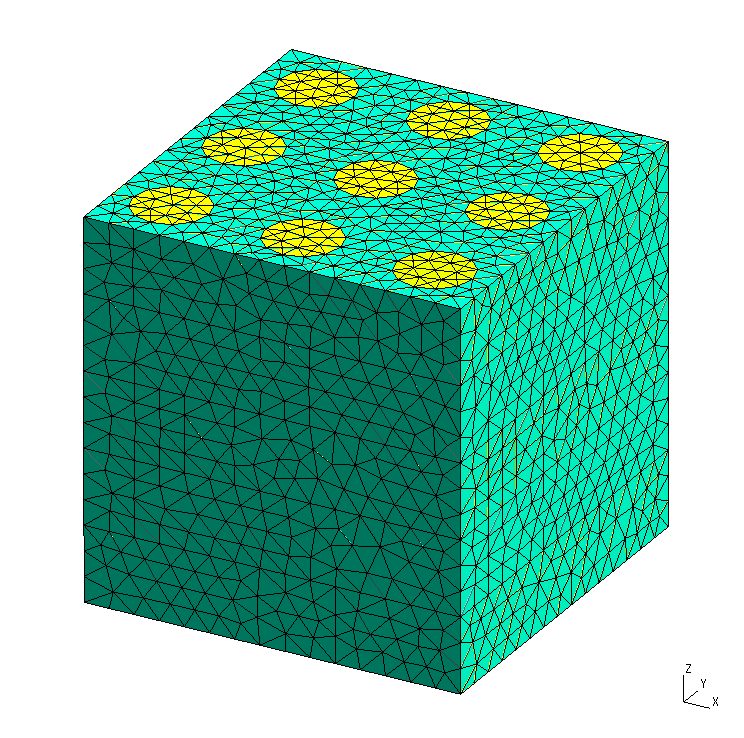
\includegraphics[scale=0.24]{fuel_z5.png}
	\end{minipage}
	\begin{minipage}{0.5\linewidth}
		\centering
		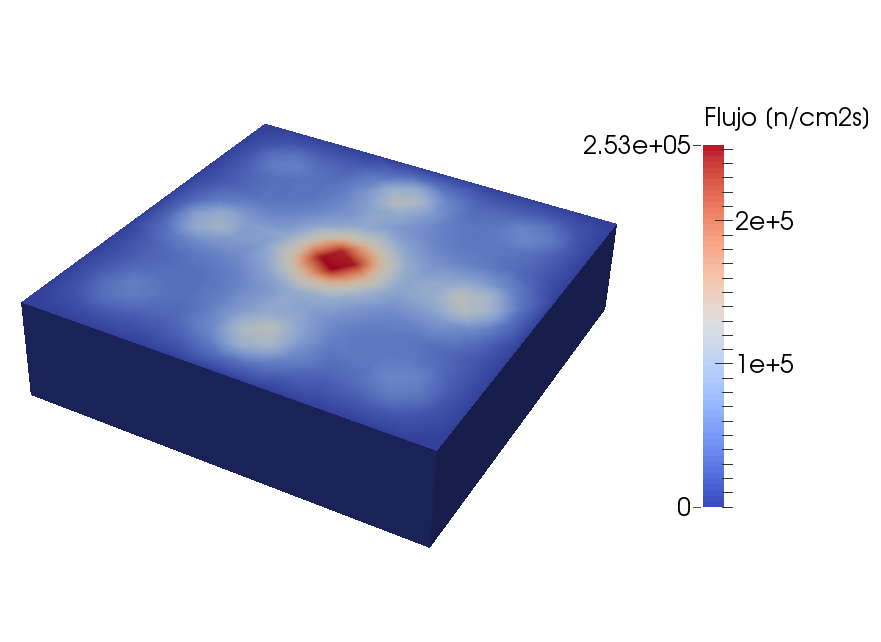
\includegraphics[scale=0.22]{flux_z5.png}
	\end{minipage}
\caption[Núcleo simple en análisis de acoplamiento neutrónico-termohidráulico utilizando \textit{RELAP5} y \textit{Fermi}]
{\textbf{(a)} Esquema de núcleo simple en análisis de acoplamiento neutrónico-termohidráulico utilizando \textbf{RELAP5} y \textbf{Fermi}.
\textbf{(b)} Distribución del flujo neutrónico obtenido en un corte axial a 0.25 $cm$ desde la base del núcleo.
}
\label{fuel_z5}
\end{figure}
El dominio de cálculo termohidráulico consiste en una simplificación de la geometría del núcleo,
considerando un único canal de refrigeración cilíndrico de sección similar a aquella por la que fluye todo el caudal del refrigerante.
Este canal está en contacto con una única estructura que genera energía, 
del mismo diámetro que el que tendrían los pines de los elementos combustibles y altura equivalente a la suma de todos ellos.
Como el modelo es ficticio, el diámetro y la cantidada de pines asumen valores arbitrarios.
La energía total generada en esta estructura es igual a la potencia total generada por el reactor. 
Este tipo de modelos es comúnmente utilizado en análsis de acoplamiento neutrónico-termohidráulico \cite{pumita-relap}.
Si bien la geometría de análisis es artificial, 
es importante contar con modelos de secciones eficaces que representen fielmente la dependencia con las variables de estado termohidráulicas.
Por este motivo se construyeron funciones de $\Sigma$ dependientes en $T_{comb}$, $T_{ref}$, $N_{ref}$ y el valor del quemado $B$
a partir de tablas de secciones eficaces proporcionadas por DIFRA (departamento de DIvisión de Física de Reactores Avanzados de CNEA).

La evolución temporal se discretiza en intervalos de 10 días.
Se definen cinco zonas axiales de acoplamiento.
Con el modelo de resolución previamente comentado, quedan definidas en total veinte incógnitas de acoplamiento.
En la Figura \ref{esquema-fermi-relap} se esquematiza la estrategia para un paso de quemado genérico.
Los mapeos entre las variables termohidráulicas y las secciones eficaces fueron implementados en la función \textit{th2xs} en el código \textit{maestro} \textbf{Newton}.
Las potencias $P_i$ calculadas por el código neutrónico son escaleadas mediante la función $P2p$ a valores $p_i$ en el cálculo de residuos.
Estos valores escaleados se definieron de tal forma que todas las variables de acoplamiento tuvieran magnitudes similares,
para evitar la construcción de matrices mal condicionadas en los métodos de resolución implícitos.
La distribución de potencias que efectivamente \textbf{Newton} envía a al código termohidráulico se define a partir de un nuevo mapeo $p2fp$
en el que se calculan las fracciones de potencia correspondientes a cada zona axial.

\pgfdeclarelayer{bg}    % declare background layer
\pgfsetlayers{bg,main}  % set the order of the layers (main is the standard laye

\begin{figure}[h]
\centering{}
\begin{tikzpicture}[
block1/.style={
	draw,
	fill=white,
	rectangle, 
	minimum width={width("Esclavo 1")+3pt},
	minimum height={17pt},
	font=\small, 
  align=center},
arrow1/.style={
  -{Latex[length=3mm, width=1mm]}
  }
]

% residuos
\node [block1, text width=6em] at (0,6em) (res) {\textbf{Resolución de residuos}};


% programa 1
\node[block1, above of=res, yshift=6em] (e1) {\textbf{Fermi}};

% alpha 1
\node [block1, below left of=e1, yshift=-0.8em, xshift=-9em] (alpha1) {$P_1, P_2, ..., P_5$};

% beta 1
\node [block1, above left of=res, yshift=0.8em, xshift=-9em] (beta1) {$p_1, p_2, ..., p_5$};

% gamma 1
\node [block1, above right of=res, yshift=0.8em, xshift=9em] (gamma1) {$N_{ref,1}, T_{ref,1}, T_{comb,1}, ..., T_{comb,5}$};

% delta 1
\node [block1, below right of=e1, yshift=-0.8em, xshift=9em] (delta1) {$\Sigma_1, \Sigma_2, ..., \Sigma_5$};


% programa 2
\node [block1, below of=res, yshift=-6em] (e2) {\textbf{RELAP5}};

% alpha 2
\node [block1, above left of=e2, yshift=2.8em, xshift=-9em] (alpha2) {$N_{ref,1}, T_{ref,1},$\\$T_{comb,1}, ..., T_{comb,5}$};

% beta 2
%\node [block1, below left of=res, yshift=-0.8em, xshift=-9em] (beta2) {$N_{ref,1}, T_{ref,1}, T_{comb,1}, ..., T_{comb,5}$};

% gamma 2
\node [block1, below right of=res, yshift=-0.8em, xshift=9em] (gamma2) {$p_1, p_2, ..., p_5$};

% delta 2
\node [block1, above right of=e2, yshift=0.8em, xshift=9em] (delta2) {$fp_1, fp_2, ..., fp_5$};

% Conexiones 1
\draw[arrow1] ($(e1.west)$) to[out=180, in=70, distance=2em] (alpha1.north);
\draw[arrow1] ($(alpha1.south)$) to node [midway, anchor=center, left]{\textit{mapeo P2p}} (beta1.north);
\draw[arrow1] ($(beta1.south)$) to[out=-70, in=-180, distance=1.7em] ($(res.west)+(0,0.2em)$);

\draw[arrow1] ($(res.east)+(0,0.2em)$) to[out=0, in=-110, distance=1.7em] ($(gamma1.south)$);
\draw[arrow1] ($(gamma1.north)$) to node [midway, anchor=center, right]{\textit{mapeo th2xs}} (delta1.south);
\draw[arrow1] ($(delta1.north)$) to [out=110, in=0, distance=2em] ($(e1.east)$);

% Conexiones 2
\draw[arrow1] ($(e2.west)$) to[out=180, in=-70, distance=2em] (alpha2.south);
\draw[arrow1] ($(alpha2.north)$) to[out=70, in=-180, distance=3em] ($(res.west)-(0,0.2em)$);
%\draw[arrow1] ($(alpha2.north)$) to node [midway, anchor=center, left]{\textit{mapeo $\alpha_2-\beta_2$}} (beta2.south);
%\draw[arrow1] ($(beta2.north)$) to[out=70, in=-180, distance=1.7em] ($(res.west)-(0,0.2em)$);

\draw[arrow1] ($(res.east)-(0,0.2em)$) to[out=0, in=110, distance=1.7em] ($(gamma2.north)$);
\draw[arrow1] ($(gamma2.south)$) to node [midway, anchor=center, right]{\textit{mapeo p2fp}} (delta2.north);
\draw[arrow1] ($(delta2.south)$) to [out=-110, in=0, distance=2em] ($(e2.east)$);

% Fondo
\begin{pgfonlayer}{bg}    % select the background layer
  % Newton frame
  \draw [blue, rounded corners, thick, dashed, opacity=0.5, fill=blue!10] 
  ($(res.west) + (-16em, 7em)$)
  -- ($(res.west) + (-16em,-7em)$)
  -- ($(res.east) + (16em,-7em)$)
  -- ($(res.east) + (16em,7em)$)
  -- ($(res.west) + (-16em,7em)$);
  % newton
  \node [draw,blue, rounded corners, thick, dashed, opacity=0.5, fill=blue!10] 
  at ($(beta1.west) + (-2em, -2.5em)$) (newton) {\textbf{Newton}};
\end{pgfonlayer}

\end{tikzpicture}
\caption[Instancias de cálculo de las variables relacionadas con cada programa \textit{esclavo}]
{Instancias de cálculo de las variables relacionadas con cada programa \textit{esclavo} en la resolución del problema de acoplamiento neutrónico-termohidráulico.
En este ejemplo los programas \textbf{Fermi} y \textbf{RELAP5} se comunican con \textbf{Newton}.}
\label{esquema-fermi-relap}
\end{figure}

El modelo neutrónico es resuelto con \textbf{Fermi} \cite{fermi}.
%\textbf{Fermi} es un código de núcleo desarrollado por Guido Giuntoli que calcula el flujo neutrónico a un grupo de energía a partir de un esquema de elementos finitos de la ecuación \ref{eq-nucleo}.
\textbf{Fermi} es un código de núcleo que calcula el flujo neutrónico a un grupo de energía a partir de un esquema de elementos finitos de la ecuación \ref{eq-nucleo}.
Las ecuaciones modelos presentadas en \ref{relap-calor}, \ref{relap-masa}, \ref{relap-momento} y \ref{relap-energia},
los modelos de cierre necesarios para formular problemas bien definidos que ajusten a los distintos regímenes de flujo,
y las ecuaciones modelos para las condiciones de borde de cada una de estas ecuaciones,
son resueltas con \textbf{RELAP5}.
\textbf{RELAP5} es un código de análisis de seguridad de reactores nucleares desarrollado por el Laboratorio Nacional de Idaho (INL por sus siglas en inglés, \textit{Idaho National Laboratory}).
\textbf{RELAP5} ha sido validado en cálculos termohidráulicos de reactores nucleares y debido al amplio uso que tiene este código a nivel internacional
se decidió utilizar en la resolución del problema modelado en la presente sección,
para demostrar la posibilidad de uso en acoplamientos mediante la estrategia descripta en el \hyperlink{chapter.2}{Capítulo 2}.
\textbf{RELAP5} resuelve las ecuaciones \ref{relap-calor}, \ref{relap-masa}, \ref{relap-momento} y \ref{relap-energia} a partir de esquemas semi-implícitos de diferencias finitas.

La resolución del sistema acoplado se llevó a cabo utilizando tres métodos diferentes.
En la Figura \ref{fig-relap-fermi} se muestra la cantidad de evaluaciones de funciones en cada paso de quemado requerida por cada método,
y la Tabla \ref{tab-relap-fermi} integra la cantidad total de evaluaciones y el tiempo consumido por cada uno.

El primer método utilizado fue el método explícito \textit{Dirichlet-to-Neumann} (iteraciones de \textit{Picard}), y es el que consume mayor tiempo de cálculo.
El segundo método utilizado es otro método explícito, el método del punto fijo.
Este método demuestra la ventaja de mantener a los diferentes programas \textit{exclavos} corriendo en paralelo.
Por último, se utilizó el método de \textit{Broyden} que en previas aplicaciones había demostrado muy buenos resultados.
Si bien este método requiere excesivas evaluaciones en la primera iteración del primer paso de cálculo para la construcción de la matriz jacobiana,
en los siguientes pasos de quemado converge con pocas iteraciones, y finalmente
este método es el que converge en la menor cantidad de tiempo.
El método de \textit{Newton-Raphson}, otros métodos \textit{quasi-Newton} como el método de la \textit{secante} o \textit{Shamanskii} y los métodos \textit{Newton-Krylov}
no fueron tenidos en cuenta puesto que hubieran requerido numerosas evaluaciones\footnote{
Si bien los recursos utilizados serían elevados,
no debería influir en el tiempo de cálculo cuando las evaluaciones solo son necesarias para la construcción de la matriz jacobiana,
puesto que este tipo de cálculo es paralelizable.
} de funciones debido a la gran cantidad de incógnitas del sistema.

\begin{minipage}{\textwidth}
\begin{minipage}[b]{0.49\textwidth}
  \centering
  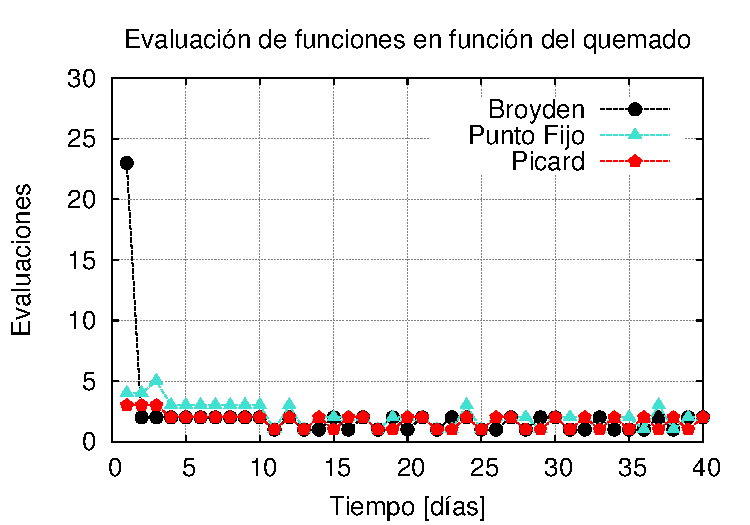
\includegraphics[scale=0.6]{fermi-relap-feval.pdf}
  \label{fig-relap-fermi}
  \captionsetup{width=0.8\textwidth}
  \captionof{figure}[Evaluaciones de funciones en cada paso de quemado en cálculo con \textbf{RELAP5} y \textbf{Fermi}]
  {Evaluaciones de funciones en cada paso de quemado en cálculo con \textbf{RELAP5} y \textbf{Fermi}.}
\end{minipage}
\hfill
\begin{minipage}[b]{0.49\textwidth}
  \centering
  \begin{tabular}{ l r r } \hline
      Método & Evaluaciones & Tiempo \\
      no lineal & totales & total [s] \\ \hline %\hline
      Picard & 68 & 684 \\ %\hline            
      Punto fijo & 87 & 628  \\ %\hline
      Broyden & 85 & 610 \\ \hline
   \end{tabular}
   \label{tab-relap-fermi}
   \captionsetup{width=0.8\textwidth}
   \captionof{table}[Evaluaciones totales y tiempo total requerido por cada método no lineal en cálculo de quemado con \textbf{RELAP5} y \textbf{Fermi}]
   {Evaluaciones totales y tiempo total requerido por cada método no lineal en cálculo de quemado con \textbf{RELAP5} y \textbf{Fermi}.}
  \end{minipage}
\end{minipage}

\subsection*{Acoplamiento neutrónico-termohidráulico utilizando RELAP y PUMA}
\label{3:relap-puma}

La segunda aplicación analizada consiste en el análisis del núcleo del reactor CAREM-25 \cite{carem} durante un ciclo de quemado de 400 días.
CAREM-25 es un reactor integrado de convección natural con generación 100 MW térmicos.
Utiliza agua liviana como refrigerante y uranio enriquecido como combustible, y
cuenta con diseños innovativos en sistemas de seguridad \cite{carem}.
El análisis de este reactor es un problema complejo, con gran cantidad de incógnitas de acoplamiento.

El dominio de cálculo neutrónico consiste en un núcleo de 1.4 metros de altura y 1.312 metros de diámetro equivalente.
Este núcleo está compuesto por 61 elementos combustibles.
Cada elemento combustible posee una sección transversal de forma hexagonal con 127 posiciones, entre las que se disponen barras con material combustible y absorbente.
En la Figura \ref{carem} puede observarse un esquema del corte axial del núcleo del reactor.

\begin{figure}

\caption[Esquema del núcleo del reactor CAREM en corte axial]
{Esquema del núcleo del reactor CAREM en corte axial.}
\label{carem}
\end{figure}
La ecuación \ref{eq-nucleo} que modela el flujo neutrónico es resuelta con \textbf{PUMA} \cite{puma} a cinco grupos de energía.
\textbf{PUMA} es un código de núcleo desarrollado por CNEA que calcula el flujo neutrónico a partir de un esquema de diferencias finitas de la ecuación \ref{eq-nucleo}.
El modelo de núcleo desarrollado para su cálculo con \textbf{PUMA} fue proporcionado por DIFRA.

El dominio de cálculo termohidráulico consiste en una simplificación de la geometría del núcleo, similar a la realizada en el ejemplo de análisis previo.
Se modela un único canal de refrigeración en contacto con una estructura de calor que contiene toda la masa de los elementos combustibles.
La longitud de esta estructura es equivalente a la longitud de la suma de todos los pines presentes en los elementos combustibles.
Radialmente, respeta la distribución de material de combustible, \textit{gap} y material de vaina.
Este modelo proviene de una monografía \cite{relap-carem} realizada durante el cursado de \textit{Modelado de sistemas termohidráulicos en reactores mediante códigos de planta}.
Las ecuaciones hidrodinámicas son resueltas con \textbf{RELAP5}.

La evolución temporal se discretiza en intervalos de 10 días.
La altura del núcleo se discretiza en tramos de 5 cm, con lo que quedan definidas 28 zonas axiales diferentes que se mantienen acopladas entre ambos modelos.
Como en cada zona axial quedan definidas cuatro incógnitas de acoplamiento, en total existen 112 incógnitas.

\begin{minipage}{\textwidth}
\begin{minipage}[b]{0.49\textwidth}
  \centering
  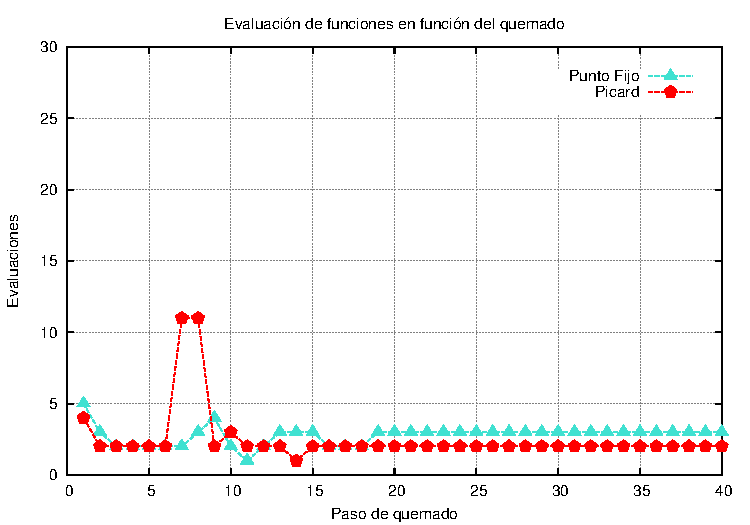
\includegraphics[scale=0.6]{puma-relap-feval.pdf}
  \label{fig-relap-puma}
  \captionsetup{width=0.8\textwidth}
  \captionof{figure}[Evaluaciones de funciones en cada paso de quemado en cálculo con \textbf{RELAP5} y \textbf{Fermi}]
  {Evaluaciones de funciones en cada paso de quemado en cálculo con \textbf{RELAP5} y \textbf{Fermi}.}
\end{minipage}
\hfill
\begin{minipage}[b]{0.49\textwidth}
  \centering
  \begin{tabular}{ l r r } \hline
      Método & Evaluaciones & Tiempo \\
      no lineal & totales & total [s] \\ \hline %\hline
      Picard & 100 & 1962 \\ %\hline            
      Punto fijo & 113 & 1614  \\ %\hline
      Broyden &  &  \\ \hline
   \end{tabular}
   \label{tab-relap-puma}
   \captionsetup{width=0.8\textwidth}
   \captionof{table}[Evaluaciones totales y tiempo total requerido por cada método no lineal en cálculo de quemado con \textbf{RELAP5} y \textbf{Fermi}]
   {Evaluaciones totales y tiempo total requerido por cada método no lineal en cálculo de quemado con \textbf{RELAP5} y \textbf{Fermi}.}
  \end{minipage}
\end{minipage}

En la resolución del sistema acoplado se consideraron solo tres métodos no lineales debido a las consideraciones comentadas en el ejemplo previo.
En la Figura \ref{fig-relap-puma} se muestra la cantidad de evaluaciones de funciones en cada paso de quemado requerida por cada método,
y la Tabla \ref{tab-relap-puma} integra la cantidad total de evaluaciones y el tiempo consumido por cada uno.

El método de \textit{Broyden} requiere numerosas iteraciones para converger en cada paso de quemado, lo que consume una excesiva cantidad de tiempo.
El método del punto fijo, presenta una ventaja frente al método de \textit{Picard}.
Debido a que el método del punto fijo posibilita el cálculo paralelo en ambos subdominios, y dado que el tiempo de cálculo consumido por cada uno de ellos es similar,
consume un tiempo de cálculo inferior para el ciclo de quemado, aún cuando la cantidad total de evaluaciones de funciones que requiere es mayor.

A pesar de que solo se estudiaron tres métodos no lineales, la estrategia de acoplamiento desarrollada provee toda la estructura necesaria para investigar nuevas propuestas.
